\graphicspath{{chapt_dutch/}{intro/}{simps/}}

% Header
\renewcommand\evenpagerightmark{{\scshape\small Chapter 6}}
\renewcommand\oddpageleftmark{{\scshape\small Search for SIMPs using Trackless Jets}}

\renewcommand{\bibname}{References}

\hyphenation{}

% STILL NEED TO CHECK ORDER OF DETAILS, OFTEN ONLY COME AFTER STATEMENT, E.G. PT DEPENDENCE OF CHF DUE TO RECO AND 1- AND 2-LEG PREDICTION.

\chapter{Search for SIMPs using Trackless Jets}
\label{ch:SIMPs}

The monojet dark matter search detailed in Chapter~\ref{ch:monojet} can be complemented at high interaction cross sections by a different search which does not look for dark matter in the form of missing transverse momentum. Indeed, if the dark matter particles have an interaction cross section of the order of the strong interaction, they will interact in the detector, mainly in the calorimeters. The analysis described in this chapter is based on this scenario, and the considered simplified model is specified in Section~\ref{sec:SIMP_model}. In this model, the dark matter particles are produced in pairs through a new strongly interacting mediator, and give rise to a pair of trackless jets as signature. Since the produced \acfp{SIMP} are neutral, the resulting jets can be distinguished from \ac{QCD} jets using the jet charged hadron energy fraction (CHF). The signal region where the \acp{SIMP} are being looked for is therefore defined by requiring the two leading jets to have a low CHF. In the control region, which is used to predict and validate the expected background, one or both jets are required to have a large CHF.

Firstly, the applied jet and photon reconstruction and identification are described, as well as the specific treatment applied for the primary vertex selection. The triggers that were designed specifically for this search, exploiting the CHF, are outlined in Section~\ref{sec:SIMP_trigger}. However, these triggers were found to be problematic and eventually a generic single jet trigger was used instead. Next, the event selection is detailed in Section~\ref{sec:SIMP_selection} for both the signal and control regions. The strategy for the background estimation and the systematic uncertainties are discussed in Sections~\ref{sec:SIMP_backgrounds} and \ref{sec:SIMP_systematics}, respectively. Finally,  in Sections~\ref{sec:SIMP_results} and \ref{sec:SIMP_interpretation}, the results are shown and interpreted in terms of the \ac{SIMP} simplified model described in Section~\ref{sec:SIMP}.

\section{Physics object reconstruction} 
\label{sec:SIMP_reconstruction}

In this analysis, jets with a very small charged hadron energy fraction (CHF) are being searched for. Since these are rather peculiar jets containing no or very few tracks, a good primary vertex selection and photon identification play an important role in suppressing the main physics and reconstruction backgrounds.

\subsection{Jets}

For the jet reconstruction, the standard method described in Section~\ref{sec:jet_reconstruction} is used. Although the jets in the signal samples are expected to be neutral, it is beneficial to use \ac{PF} jets because they directly provide an unambiguous association of tracks to jets. The standard jet energy corrections are applied as well, while the standard jet identification criteria are not used, since several of the quality criteria would actually remove the neutral \ac{SIMP} jets.

\subsection{Photons}

Since photons might be reconstructed as neutral jets, photon + jets events are an important background for the control as well as the signal region. The photons therefore need to be identified and rejected, which is done using the standard photon loose identification described in Section~\ref{sec:electron_ID}. Further photon rejection is achieved by analysis-specific selections on photon conversions and on the jet neutral electromagnetic energy fraction (NEMF), as described in Section~\ref{sec:SIMP_selection}.

\subsection{Primary vertex}

% In the standard primary vertex reconstruction, the vertex with the highest $\sum p_T^2$ is chosen, where the sum runs over the tracks associated to the vertex following the application of a deterministic annealing filter which assigns weights to sufficiently high-quality tracks that enter the vertex fit~\cite{Chatrchyan:2014fea}. While in events with jets many tens of high-momentum tracks can usually be associated to a primary vertex, thus making primary vertex finding almost fully efficient and pure, in the case of a pair of neutral jets this is not the case any more. The underlying event and potentially initial state \ac{QCD} radiation can still provide some tracks, but in extreme cases a wrong vertex is chosen, arising from a hard pileup collision.

The standard primary  vertex reconstruction described in Section~\ref{sec:tracking} sometimes provides a wrong primary vertex, which arises from a pileup interaction. The choice of a wrong vertex is not a problem in the case of signal events, which will pass in particular the CHF cuts in the event selection detailed in Section~\ref{sec:SIMP_selection} just as easily. However, a wrongly chosen vertex in a \ac{QCD} background event leads to the jets having an artificially very low CHF, both in simulation and data, as the standard \acf{CHS} procedure will remove the tracks from the vertex of the true hard interaction. This makes such events appear signal-like. For the lowest jet charged hadron energy fractions considered in this analysis, this background of events with a misidentified primary vertex becomes dominant with respect to the background from \ac{QCD} events with a very rare jet fragmentation into predominantly neutral hadrons and photons. In Figure~\ref{fig:wrongvertex} an event display is shown that demonstrates such a wrong choice of vertex.

\begin{figure}[ht]
  \centering
  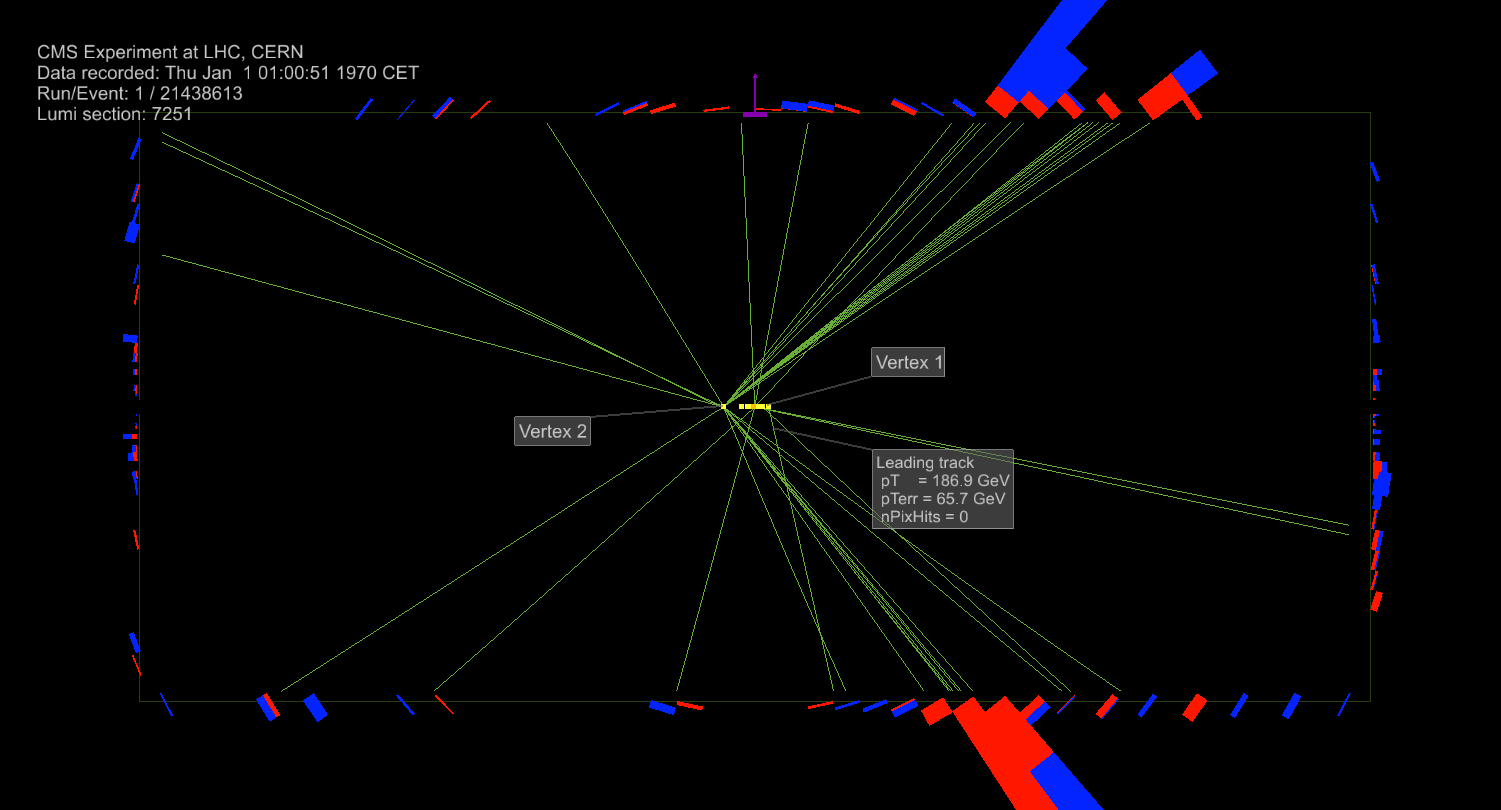
\includegraphics[width=0.99\textwidth]{figures/wrongvertex.png}
  \caption{Event display showing an example of a wrong primary vertex selection in a MC simulated \ac{QCD} event. Although "Vertex 2" is the real vertex of the hard collision, "Vertex 1" is selected because of the presence of a single high-$p_T$ track with poor momentum resolution and no pixel hits attached. As a result, the two visible high-$p_T$ jets (above \SI{200}{GeV}), clearly with many tracks attached, are reconstructed with only 3\% and 4\% of charged energy fraction.}
  \label{fig:wrongvertex}
\end{figure} 

Investigating this problem, many events with a wrong vertex assignment were observed to have the highest-$p_T$ track being of poor quality, with a high momentum with large uncertainty, and no pixel hits. This alone, though, does not provide a sufficient handle to suppress this background, and a plain cut on number of pixel hits was verified to remove a lot of signal events as well.
% plot or numbers to show reduction in signal?
Studying the simulated \ac{QCD} multijet events with a very low CHF coming from primary vertex misidentification by analysing event displays also showed that the true vertex is reconstructed as the second vertex in the list for the far majority of the cases. A second jet reconstruction was therefore produced, based on selecting the second entry in the list of primary vertices to be the event's collision vertex, and rerunning the \ac{CHS} as well. If this second vertex was the correct one, the jets will now have a large CHF in most of the cases, while the first event reconstruction yields low-CHF jets. In the event selection discussed in Section~\ref{sec:SIMP_selection}, it is then sufficient to ask both event reconstructions to pass the cut of low jet CHF, effectively suppressing this background induced from wrong primary vertex selection.

\section{Trigger selection}
\label{sec:SIMP_trigger}

Several triggers have been designed specifically for this analysis, as shown in Table~\ref{tab:triggers}. Four triggers were available to select signal events, denoted as ``signal'' in the table and providing a trade-off between a high CHF and a low jet $p_T$. The CHF cut is always applied on both jets. Two additional triggers, indicated with the ``control'' type, were used to determine the trigger efficiencies. These triggers were prescaled, meaning that only a fraction of the events are kept due to the otherwise very high rate of the trigger.

\begin{table}[ht]
  \centering
  \begin{tabular}{| l | c | c |}
    \hline
    Trigger name & Type & Int. Lumi. \\
    \hline
    \verb|HLT_DiCentralPFJet170_CFMax0p1_v*|     & Signal  & $33.1 \, \mathrm{fb}^{-1}$ \\
    \verb|HLT_DiCentralPFJet220_CFMax0p3_v*| \tablefootnote{Due to the unexpected high rate, this trigger was disabled after some time.}    & Signal  & $5.91 \, \mathrm{fb}^{-1}$ \\
    \verb|HLT_DiCentralPFJet330_CFMax0p5_v*|     & Signal  & $33.1 \, \mathrm{fb}^{-1}$ \\
    \verb|HLT_DiCentralPFJet430_v*|              & Signal  & $33.1 \, \mathrm{fb}^{-1}$ \\
    \verb|HLT_DiCentralPFJet170_v*|              & Control & $0.101 \, \mathrm{fb}^{-1}$ \\
    \verb|HLT_SingleCentralPFJet170_CFMax0p1_v*| & Control & $0.375 \, \mathrm{fb}^{-1}$ \\
    \hline
  \end{tabular}
  \caption{Summary of the triggers designed for this analysis, with the corresponding integrated luminosity collected for each trigger.}
  \label{tab:triggers}
\end{table}

These triggers were designed to select events containing jets with a low CHF, but keeping the jet $p_T$ threshold as low as possible, while taking the limited trigger rate into account. Their performance was tested using simulated \ac{QCD} events before using them in data taking. The trigger efficiency of \texttt{HLT\_DiCentralPFJet330\_CFMax0p5} as a function of $p_{T}$ and CHF is shown in Figure~\ref{fig:efficiencies_qcd_data}, using data and simulated \ac{QCD} events. The plot on the left shows the efficiency as a function of $p_T$, which quickly reaches a plateau at 100\% around \SI{350}{GeV}, as expected. The efficiency as a function of CHF is shown on the right and also shows a plateau at 100\% for low CHF. The slope of the turn-on is however less steep and only reaches the plateau around 0.35, for a threshold at CHF = 0.5 at trigger level. The signal efficiency measurement was first tried by taking a photon + jet sample, as photons could also mimic neutral jets. The photon was matched to the leading jet within a $\Delta R$ cone, and the efficiency was measured at low CHF. However, as the jet is reconstructed with a large electromagnetic energy fraction (EMF) and it does not mimic the \ac{SIMP} signal. 

\begin{figure}[ht]
  \centering
  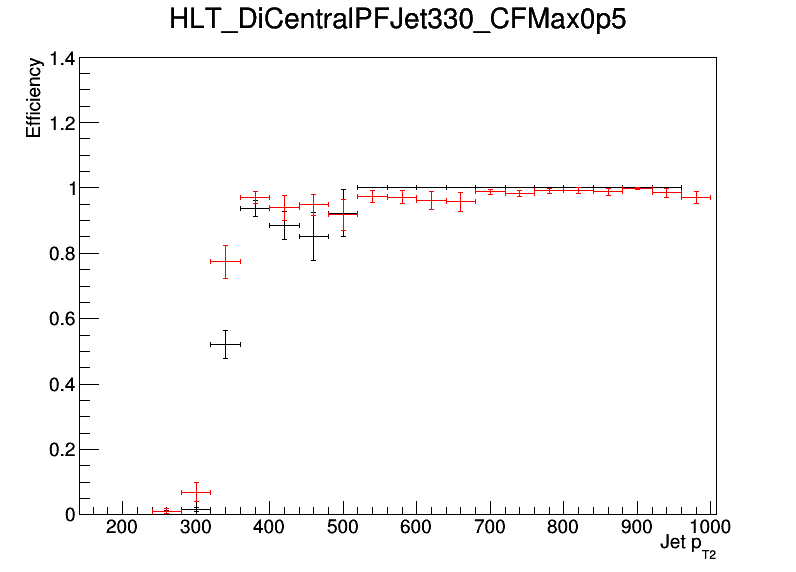
\includegraphics[width=0.47\textwidth]{figures/trigger/pt_eff_05_DataMC.png}\hfill%
  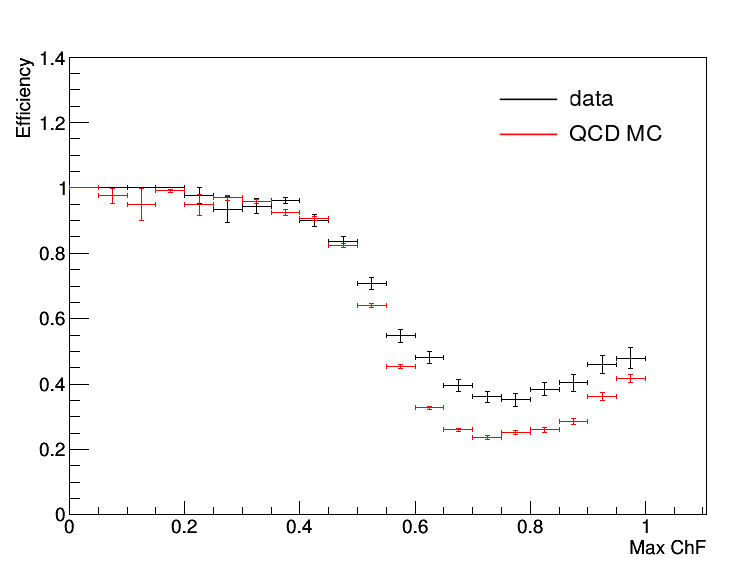
\includegraphics[width=0.47\textwidth]{figures/trigger/chf_eff_05_DataMC.png}
  \caption{The \texttt{HLT\_DiCentralPFJet330\_CFMax0p5} trigger efficiency as a function of $p_{T}$ (left) and CHF (right). Comparison between data (black) and \ac{QCD} simulation (red). }
  \label{fig:efficiencies_qcd_data}
\end{figure}

Instead, one of the neutron signal samples described in Section~\ref{sec:SIMPs} was used, generated with a \ac{SIMP} mass of \SI{700}{GeV}. The obtained trigger efficiency as a function of $p_{T}$ and CHF is shown in Figure~\ref{fig:efficiencies_simp_data} for \texttt{HLT\_DiCentralPFJet330\_CFMax0p5}, comparing the data and the signal-like events. This shows that the trigger reaches a plateau at only 60\% signal efficiency. The origin of the inefficiency was found to come from a hidden requirement asking at least one charged particle in the jets. This explains why the trigger efficiencies turn on at the expected values when using data or simulated \ac{QCD} events, where jets nearly always contain some tracks, while it is largely inefficient in signal-like simulation which generates neutral jets.

\begin{figure}[ht]
  \centering
  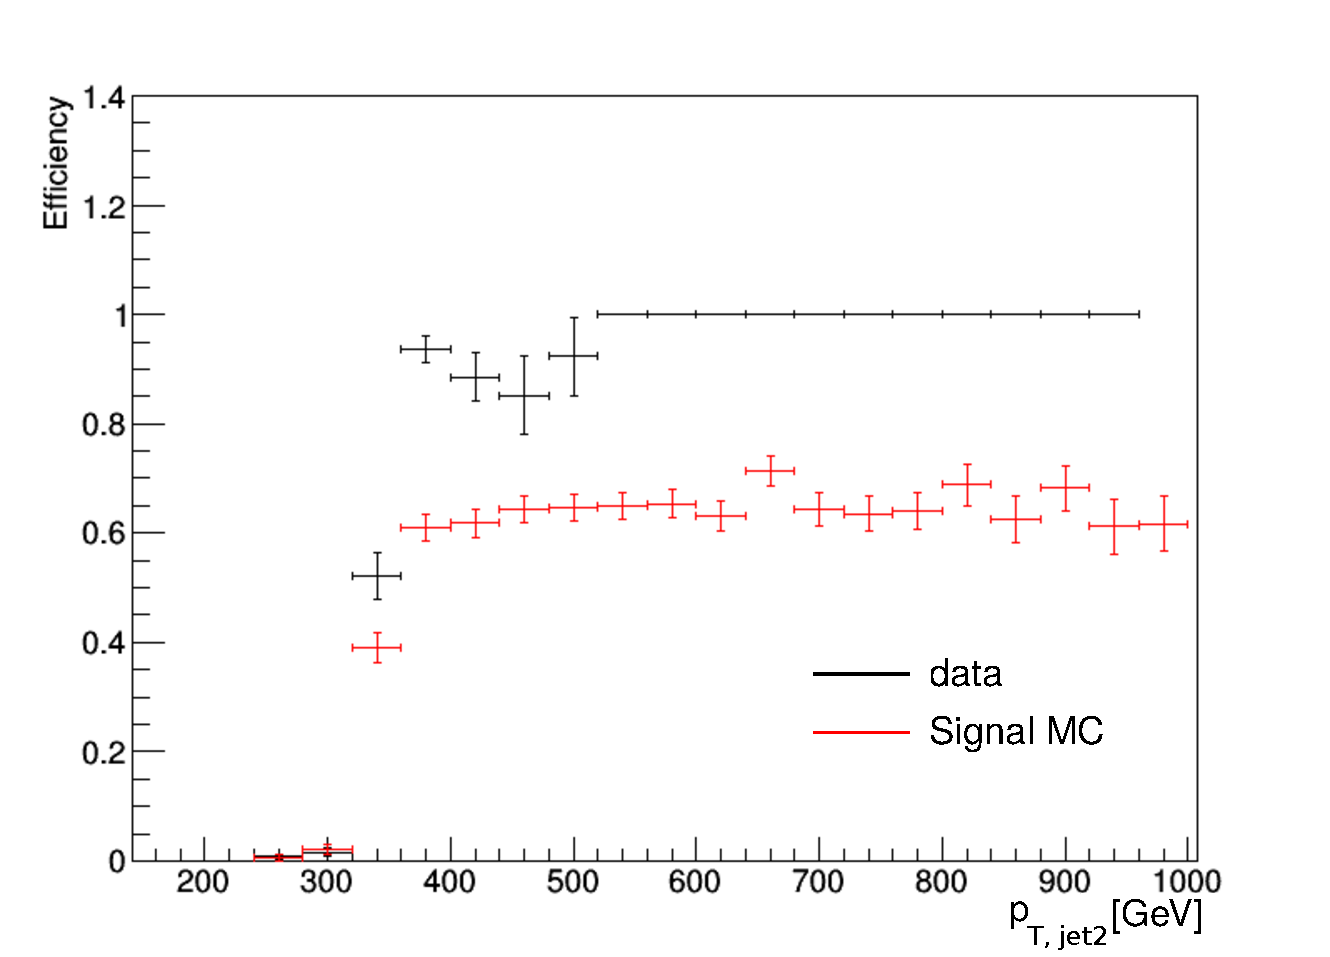
\includegraphics[width=0.47\textwidth]{figures/trigger/pt_eff_05_DataSIMP.pdf}\hfill%
  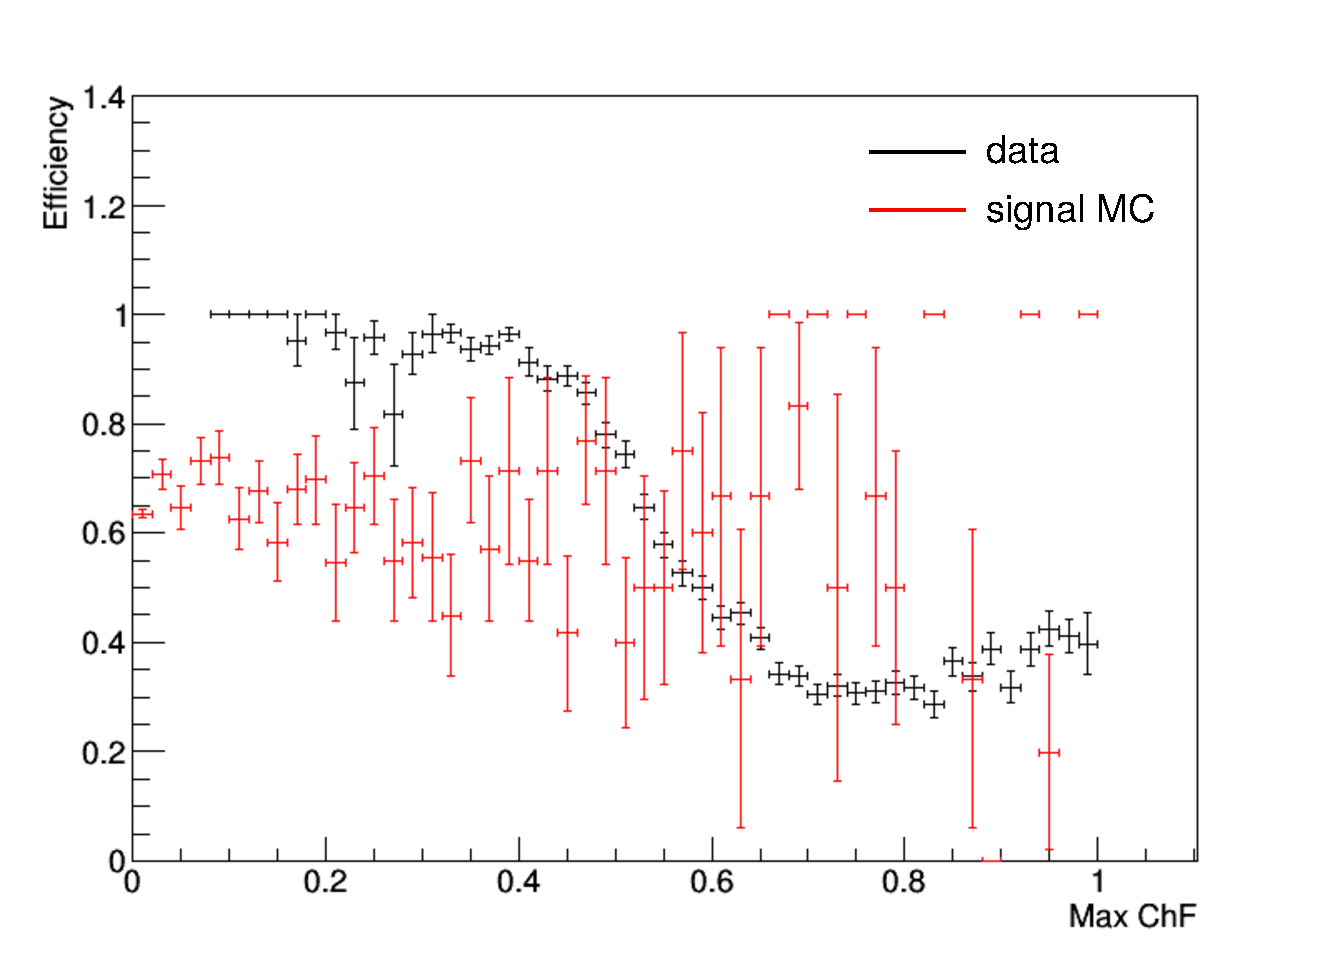
\includegraphics[width=0.47\textwidth]{figures/trigger/chf_eff_05_DataSIMP.pdf}
  \caption{The \texttt{HLT\_DiCentralPFJet330\_CFMax0p5} trigger efficiency as a function of $p_{T}$ (left) and CHF (right). Comparison between data (black) and signal-like MC (red).}
  \label{fig:efficiencies_simp_data}
\end{figure}

After this problem had been uncovered, the single jet trigger \texttt{HLT\_PFJet450} has been used for the analysis. It was selected because it has the lowest threshold among the unprescaled\footnote{Triggers with a lower $p_T$ threshold exist, but these are prescaled. Prescaled triggers are typically not used to perform an analysis, as only a small fraction of the events that pass the trigger are kept, leading to large statistical uncertainties.} single jet triggers. The trigger efficiency for the data was measured using single muon events, and is defined as
\begin{equation}
\epsilon = \frac{\mathrm{Obs}(\texttt{HLT\_PFJet450}\ \mathrm{and}\ \texttt{HLT\_IsoMu24})}{\mathrm{Obs}(\texttt{HLT\_IsoMu24})},
\end{equation} 
where Obs in this case is the $p_T$ spectrum of the leading jet for events that fired the single muon (and single jet) trigger. The jets are required to have a muon energy fraction smaller than $0.3$ in order to avoid jets with large difference in the online and offline $p_T$. This difference can arise when the offline \ac{PF} jet contains a high-$p_T$ muon. Since the online jet is reconstructed using only information from the calorimeters, this can significantly change the total $p_T$ of the jet between online and the offline \ac{PF} jet. The trigger efficiency was also measured in the simulated \ac{QCD} and neutron signal samples. In this case the denominator is the $p_T$ spectrum of leading jet without any trigger selection, while the numerator is the $p_T$ spectrum of the events firing the single jet trigger. Figure~\ref{fig:ptturnon} shows the turn-on curves for data, \ac{QCD} events, and the signal-like events. The trigger efficiency was found to be $98\%$ for jets with $p_{T}>\SI{550}{GeV}$.

\begin{figure}[ht]
  \centering
  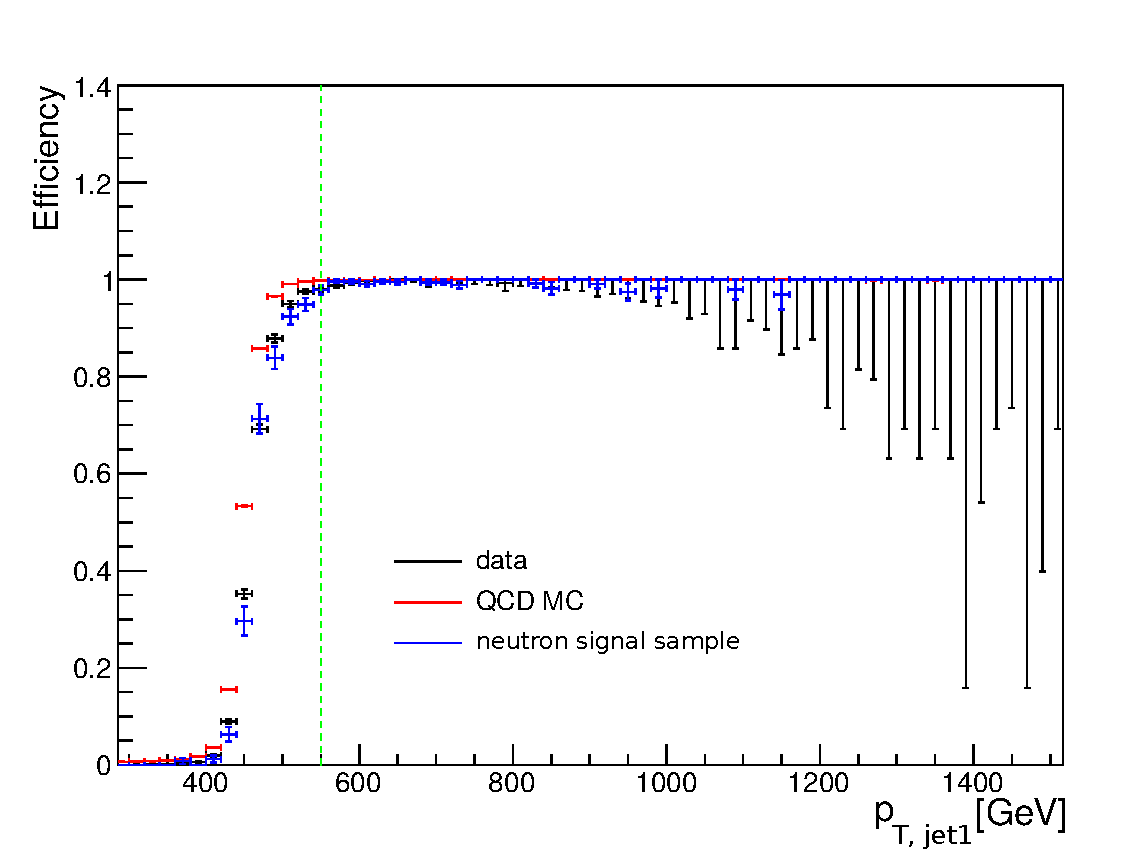
\includegraphics[width=0.7\textwidth]{figures/trigger/pt_HLT_PFJet450_new.pdf}
  \caption{The \texttt{HLT\_PFJet450} trigger efficiency turn-on as a function of the offline leading jet $p_T$, for data, \ac{QCD} events, and the signal-like events. The $p_T$ cut used in the event selection is shown with a green dashed line.}
  \label{fig:ptturnon}
\end{figure}

\section{Event selection}
\label{sec:SIMP_selection}

The event selection aims to select back-to-back dijet events with a low CHF. As a baseline selection, the two highest-$p_T$ jets are required to have $p_T > \SI{550}{GeV}$, in order to ensure the jets to be above the turn-on of the trigger. Furthermore, they are required to have $|\eta| < 2.0$, placing them fully within the tracking volume, thus suppressing backgrounds from jets that have a low CHF due to tracks falling out of tracker acceptance. Since the \acp{SIMP} do not undergo parton showering, while \ac{QCD} partons undergo final state radiation, events with \acp{SIMP} have a lower number of jets than \ac{QCD} multijet events, as can be seen from the top right plot in Figure~\ref{fig:event_selection_2}. Events containing additional jets with $p_T>\SI{30}{GeV}$ in the full $\eta$ acceptance of the CMS calorimeters on top of the two leading jets are therefore vetoed.

A photon veto is also applied to suppress photon + jets events. This is done by rejecting events with a photon within $\Delta R < 0.1$ of the leading or subleading jet, using the loose working point of the cut-based photon identification to identify photons, as described in Section~\ref{sec:electron_ID}. In some cases, however, jets have a large photon energy fraction, but the photon in the jet does not pass the loose identification requirements, for instance when there is a photon conversion in the tracker. In order to reject photon + jets events more efficiently, an additional cut is applied, as described in Section~\ref{sec:electron_ID}.
%when the jet photon energy fraction is greater than $0.8$ and the photon in the jet does not pass the loose identification. The events are rejected if conversions with $p_{T,conv} / p_{T,\gamma} > 0.3$ are matched to the photon within $\Delta R < 0.2$. In addition, the 2 jets are required to have a neutral electromagnetic energy fraction lower than 0.9, corresponding to one of the standard tight jet identification requirements mentioned in Section~\ref{sec:jet_reconstruction}. The full jet ID is not applied, since the requirements on e.g. the neutral hadronic energy fraction and the charged multiplicity would reject the signal events.

In order to avoid any problems related to the striking discrepancy between data and simulation observed for events with only one reconstructed vertex in the top left plot of Figure~\ref{fig:event_selection_2}, at least two reconstructed vertices are required. Additionally, the azimuthal separation of the two selected jets is required to be $\Delta\phi > 2$ in order to obtain back-to-back jets, which rejects the peak visible in data at $\Delta\phi = 0$ in the bottom left plot of Figure~\ref{fig:event_selection_2}. Finally, noise filters are applied in order to reject beam halo or instrumental background, such as noise in the calorimeters.

Table~\ref{tab:cutflow} shows the number of events remaining in data, for simulated \ac{QCD} events, and for 2 signal samples, after consecutively applying the described selection cuts. This shows that the background is already reduced by a factor 5, mainly by the cut on the number of jets, while a high efficiency is maintained for the signal. In Figure~\ref{fig:event_selection}, data, \ac{QCD} multijet simulation, and signal are compared after these selections, for the $p_T$, $\eta$ and CHF of the two leading jets. Figure~\ref{fig:event_selection_2} shows the distribution of the number of vertices, the number of jets, $\Delta\phi(\mathrm{jet}1, \mathrm{jet}2)$, and $H_{T}$, which is defined as the scalar sum of the transverse momenta of the two jets. In some cases, all the selection cuts except the cut on the variable being shown are applied. The bump and long tail that can be seen in the data for the $\Delta\phi(\mathrm{jet}1, \mathrm{jet}2)$ distribution contain events coming from processes with a heavy vector boson, such as Z + jets or W + jets, or $t\bar{t}$ events. The simulation instead shows a steeply falling spectrum since only \ac{QCD} dijet events are shown. Contributions from Z + jets or W + jets, and $t\bar{t}$ events were verified to be negligible in the signal region using simulated samples.

\renewcommand{\arraystretch}{1.4}
\begin{table}[ht]
  \centering
\begin{tabular}{| l | r | r | r | r |}
\hline
\multirow{2}{*}{selection cut} & \multicolumn{4}{ c |}{yield}\\
\cline{2-5}
 & \multicolumn{1}{c|}{data} & \multicolumn{1}{c|}{QCD MC} & SIMP ($m_{\chi} = 1$ GeV) & SIMP ($m_{\chi} = 1000$ GeV) \\
 \hline
$p_T^{j1, j2}>550$ GeV & 2540420 & 3152550 & 773 & 5.7 \\
$|\eta_{j1, j2}|<2.0$ & 2441240 & 2980320 & 748 & 5.6 \\
\# jets = 2 & 534053 & 587670 & 636 & 4.9 \\
photon veto & 531366 & 586674 & 636 & 4.9 \\
\# vertices $\geq$ 2 & 531244 & 586641 & 636 & 4.9 \\
 $\Delta\phi(j1, j2) > 2$ & 531207 & 586641 & 636 & 4.9 \\
noise filters & 528614 & 582184 & 634 & 4.9 \\
\hline
\end{tabular}
\caption{Number of events remaining after the listed selection cuts in data, QCD events, and 2 signal samples.}
\label{tab:cutflow}
\end{table}

\begin{figure}[ht]
  \centering
  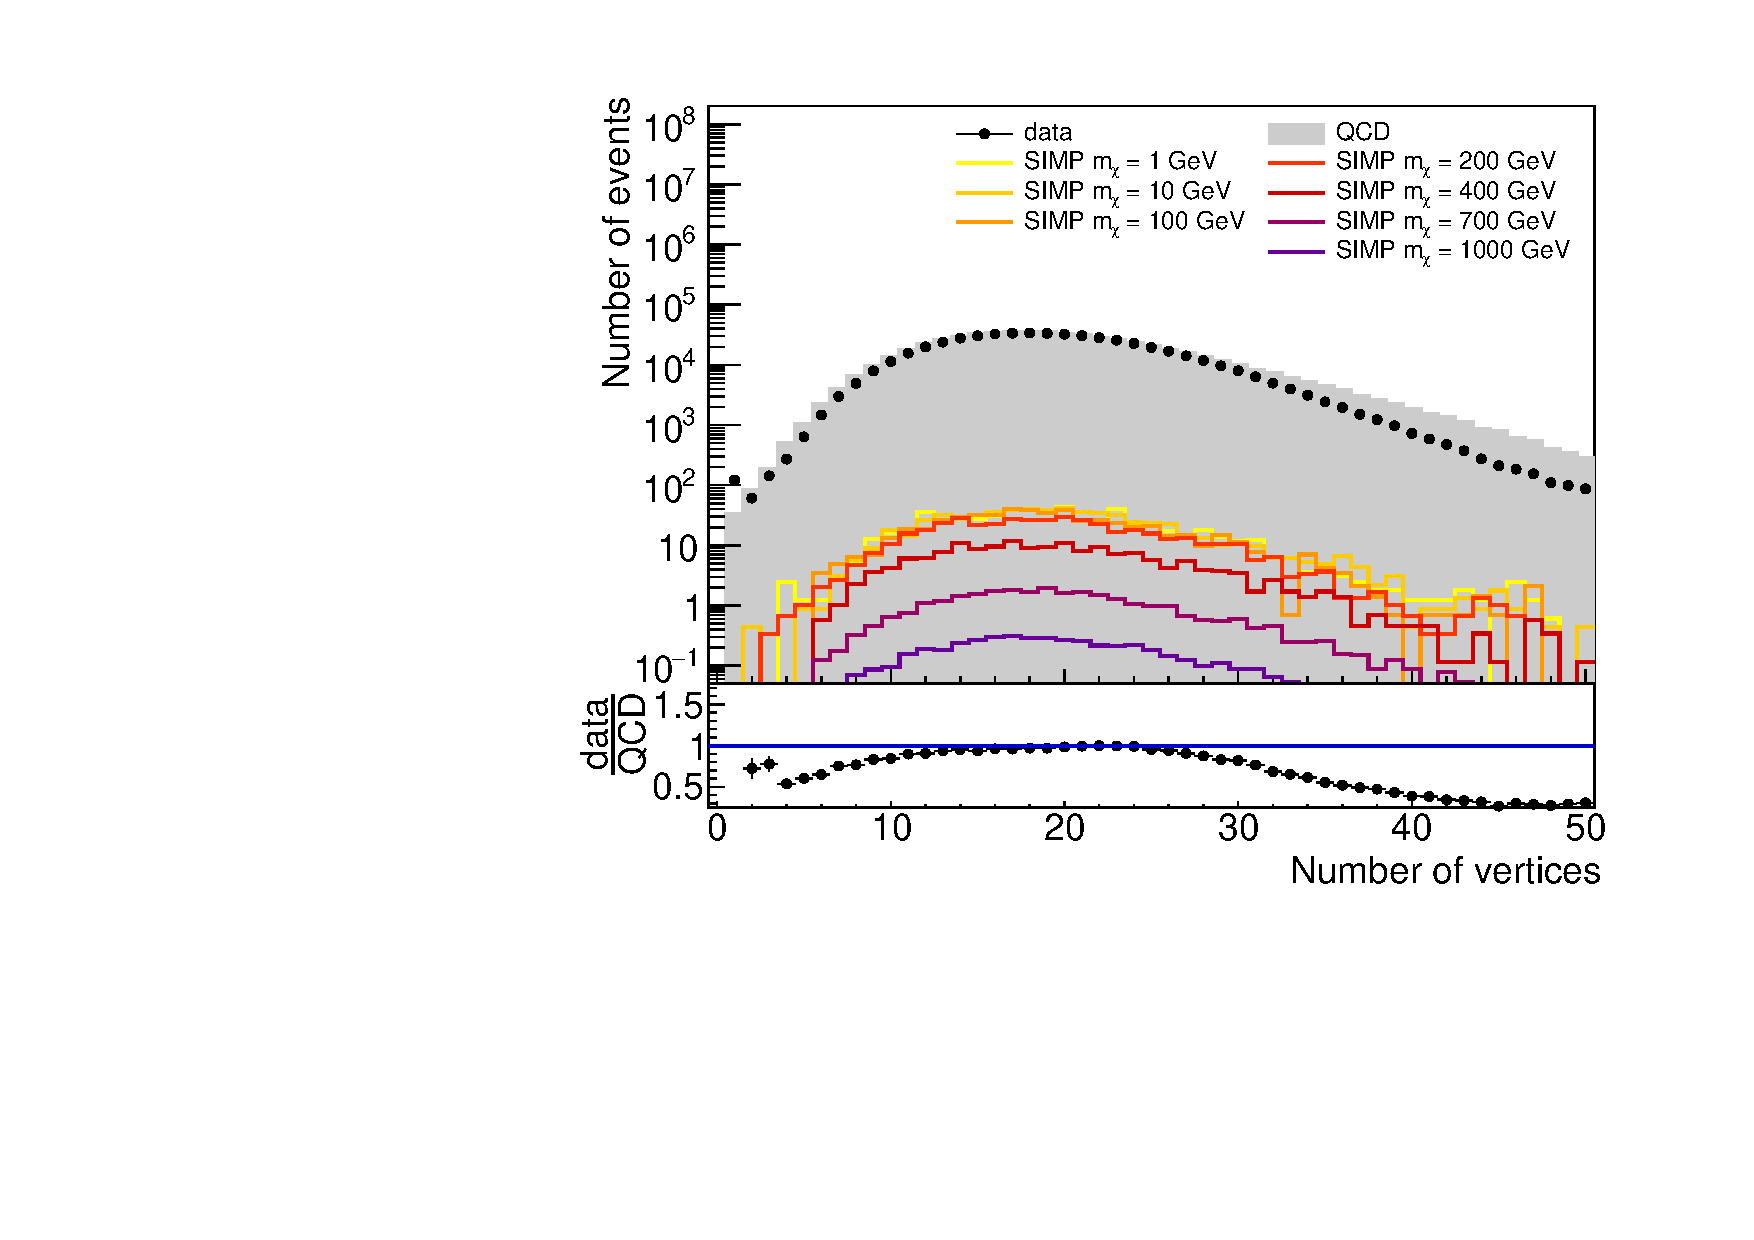
\includegraphics[width=0.5\textwidth]{figures/nvtx_newtrigger}\hfill%
  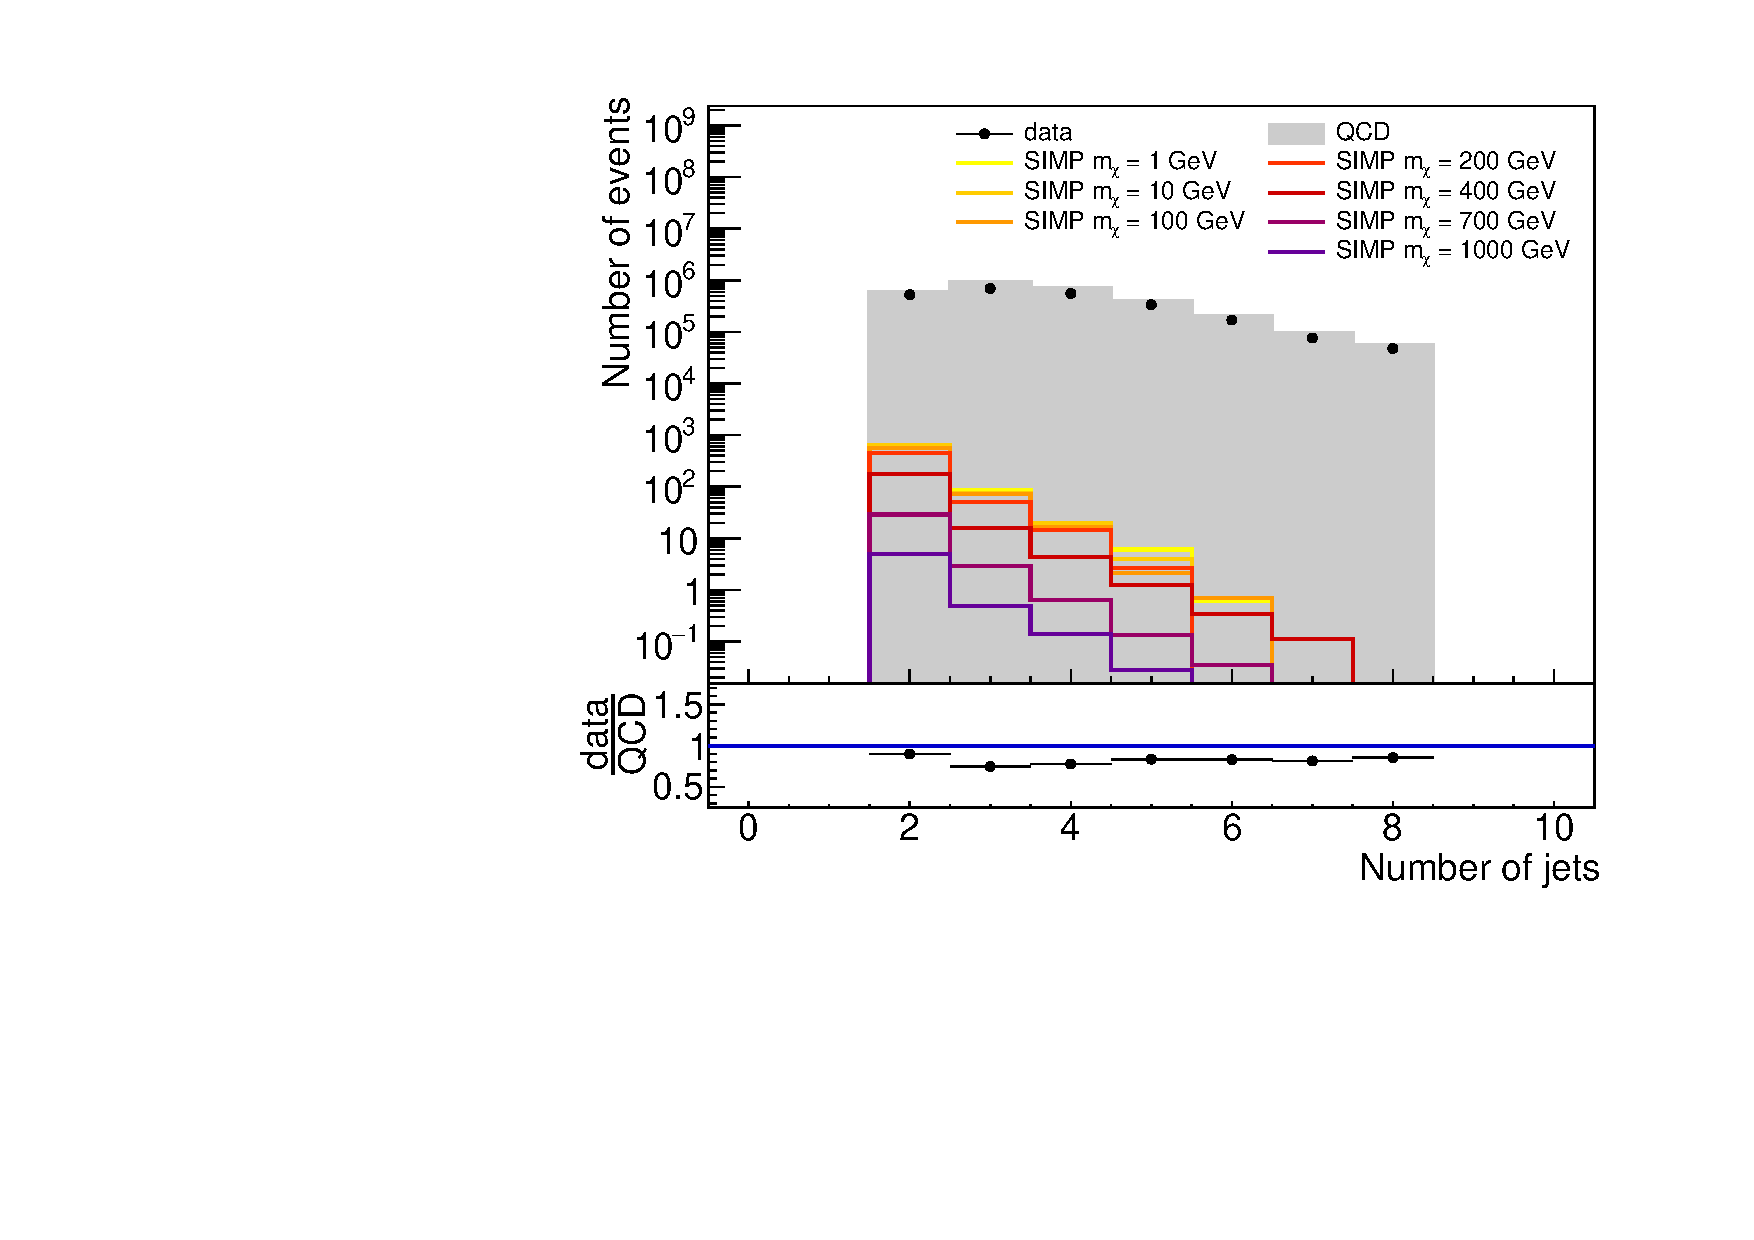
\includegraphics[width=0.5\textwidth]{figures/njets_newtrigger}
  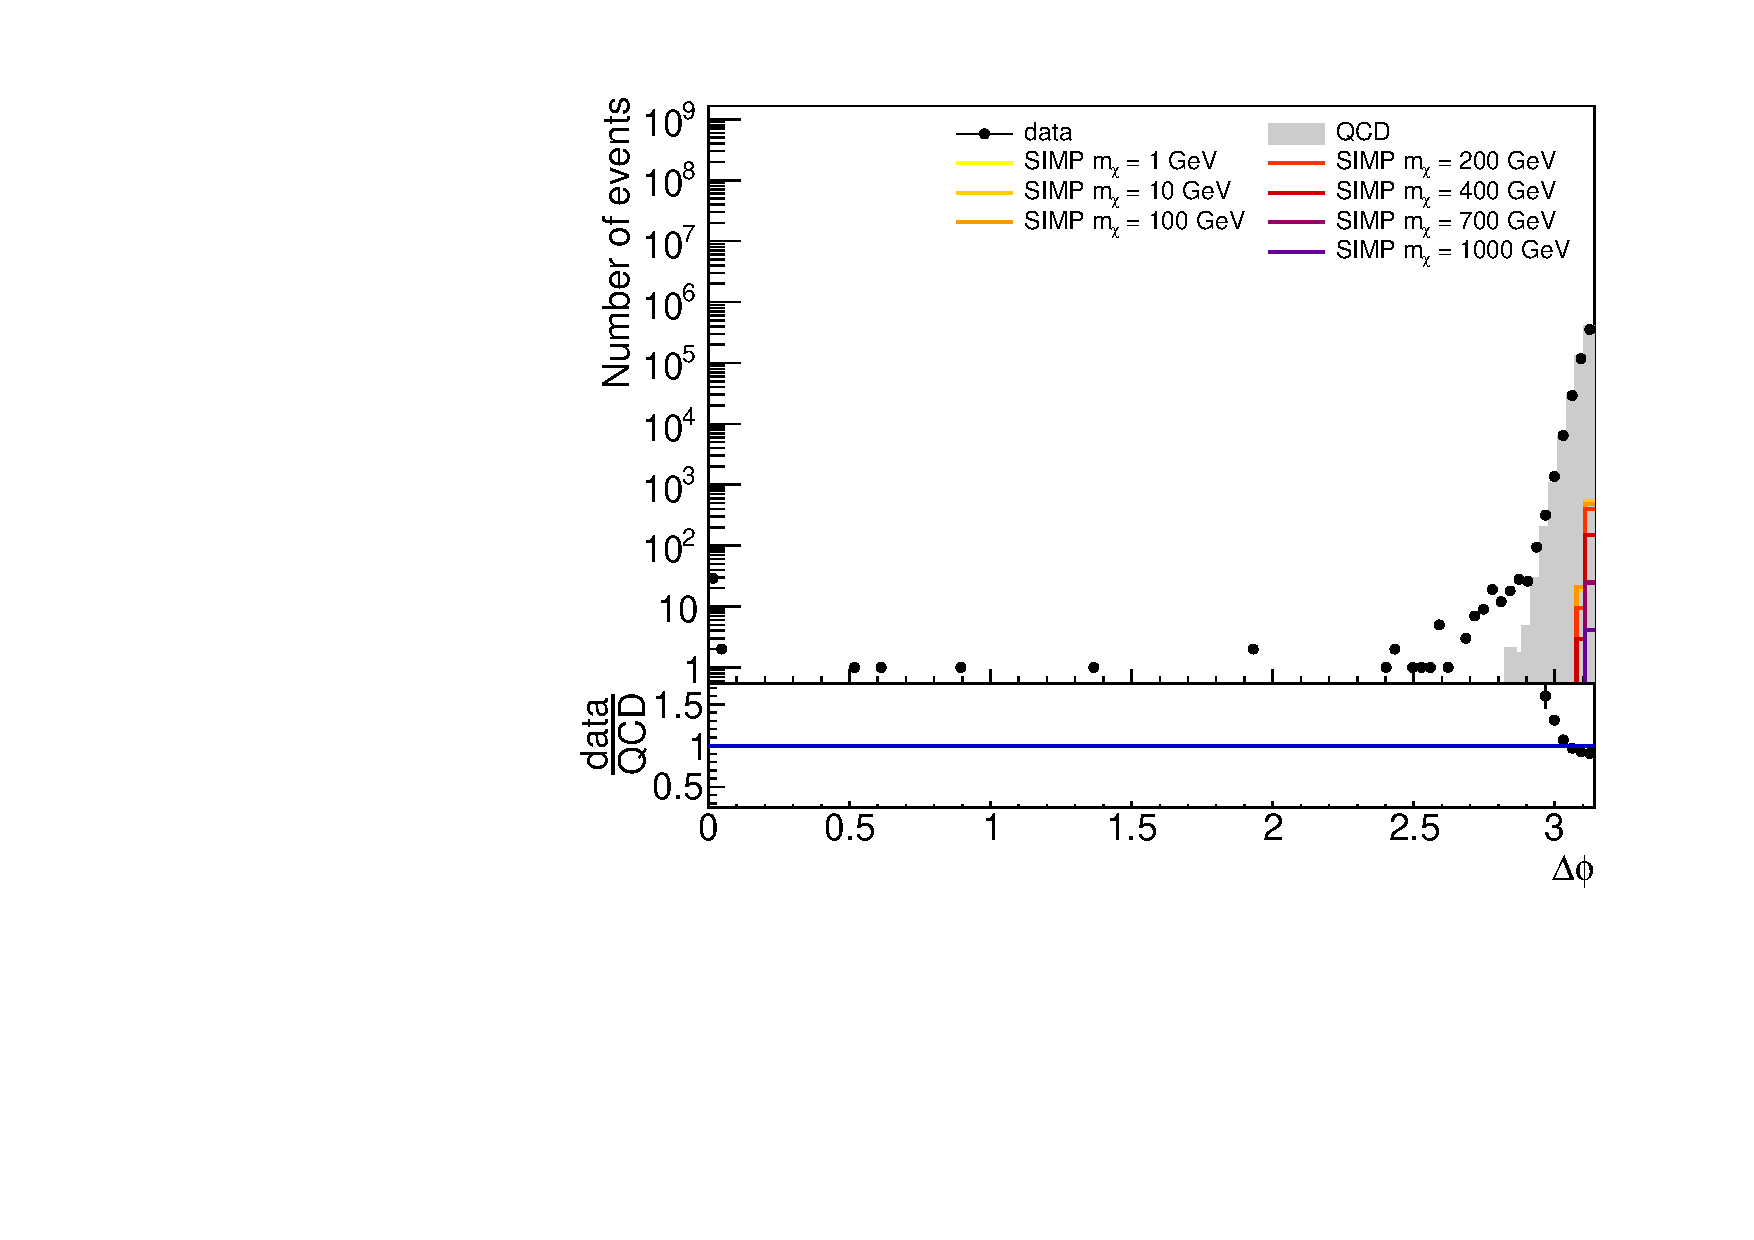
\includegraphics[width=0.5\textwidth]{figures/deltaphi}\hfill
  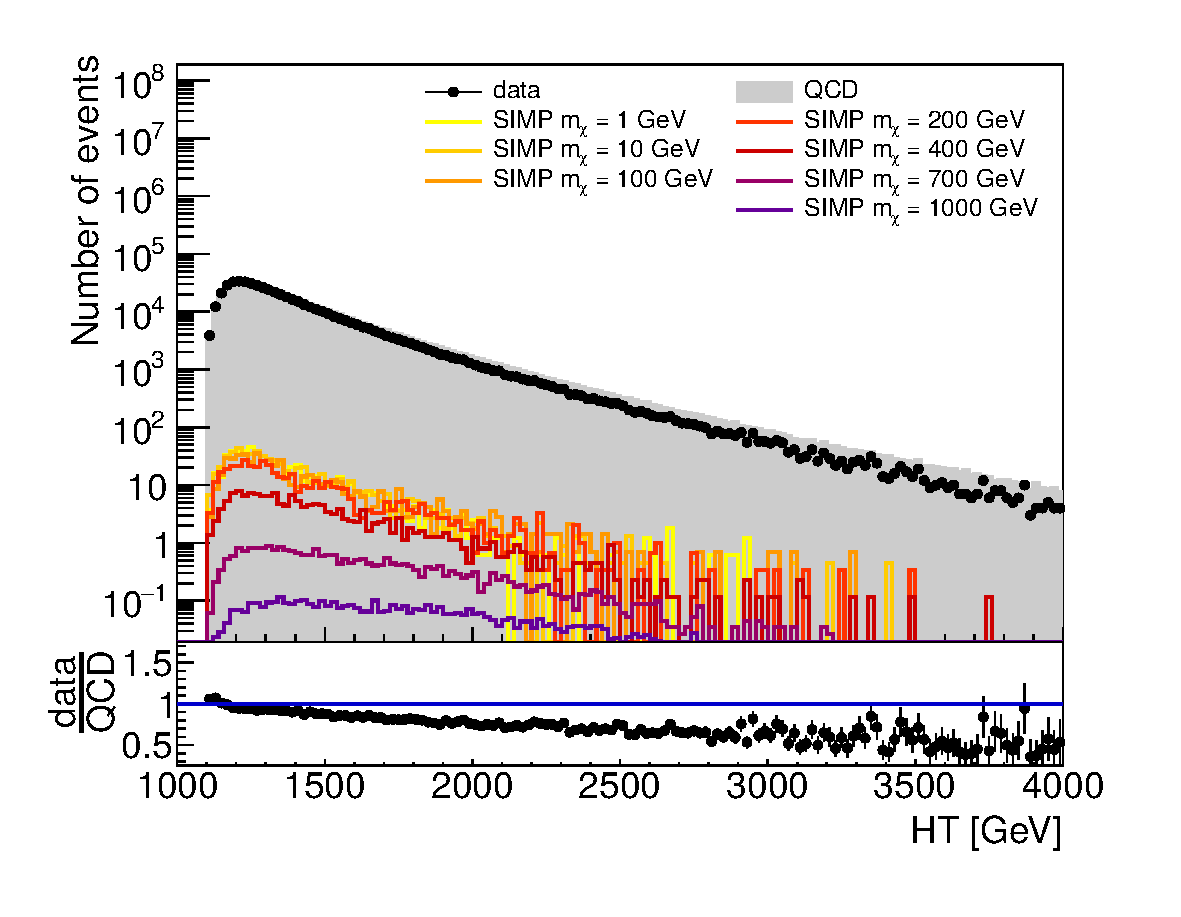
\includegraphics[width=0.5\textwidth]{figures/HT_newtrigger}
  \caption{Number of vertices, number of jets in the full detector acceptance with $p_T > \SI{30}{GeV}$, $\Delta\phi (\mathrm{jet}1, \mathrm{jet}2)$, and $H_{T}$ distributions, with selection cuts applied. The requirement on the number of vertices is not applied for the corresponding plot, the cut on the number of jets is not applied for the number of jets distribution, and the $\Delta\phi$ cut is similarly not applied for the corresponding distribution.}
  \label{fig:event_selection_2}
\end{figure}

\begin{figure}[ht]
  \centering
  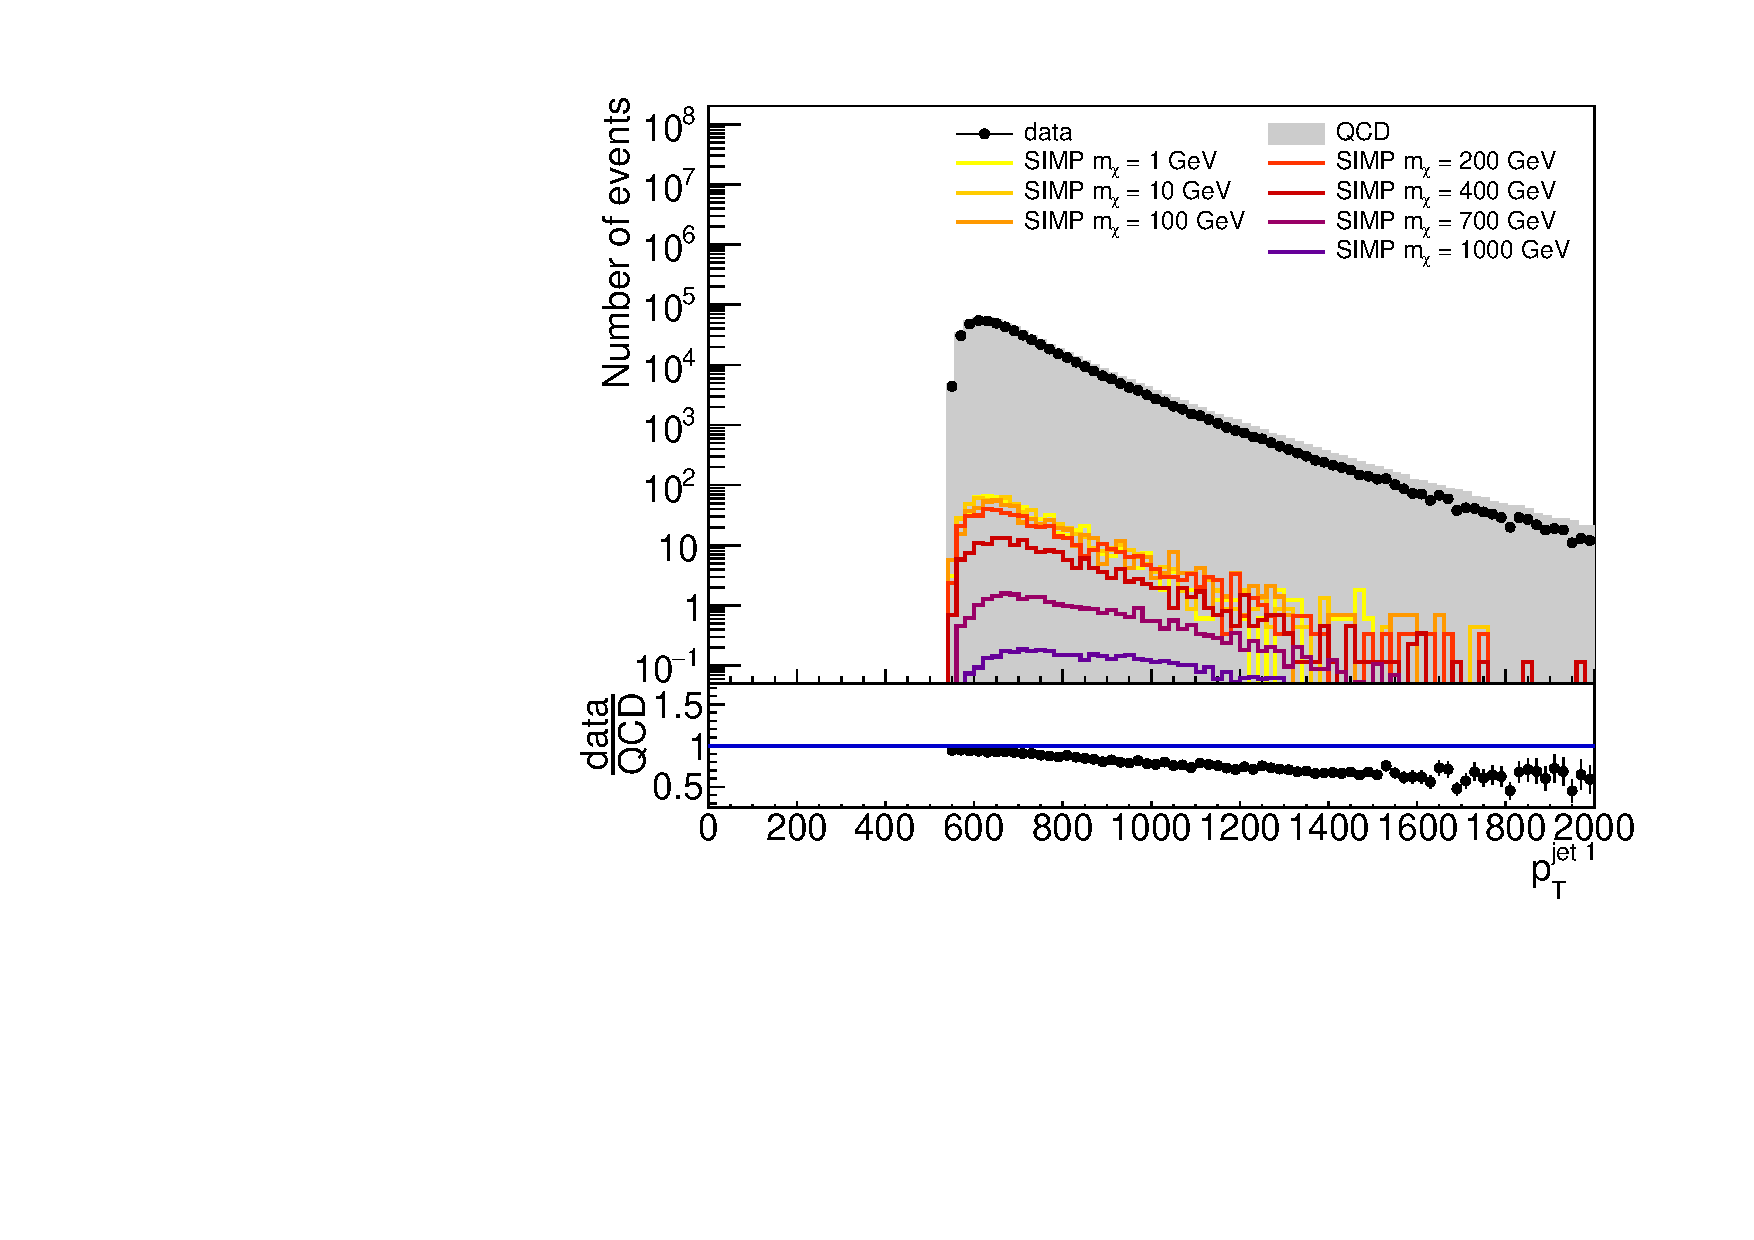
\includegraphics[width=0.5\textwidth]{figures/jet1_pt_newtrigger}\hfill%
  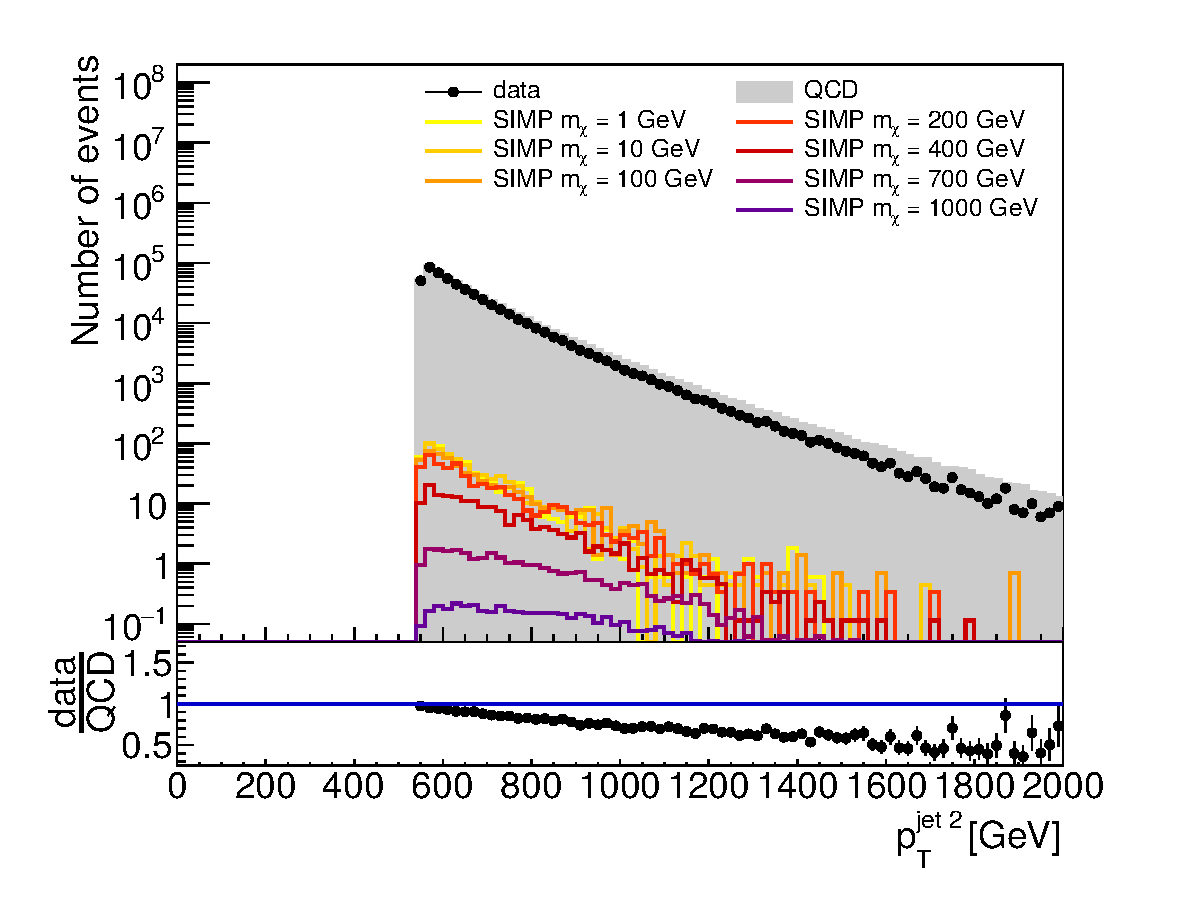
\includegraphics[width=0.5\textwidth]{figures/jet2_pt_newtrigger}
  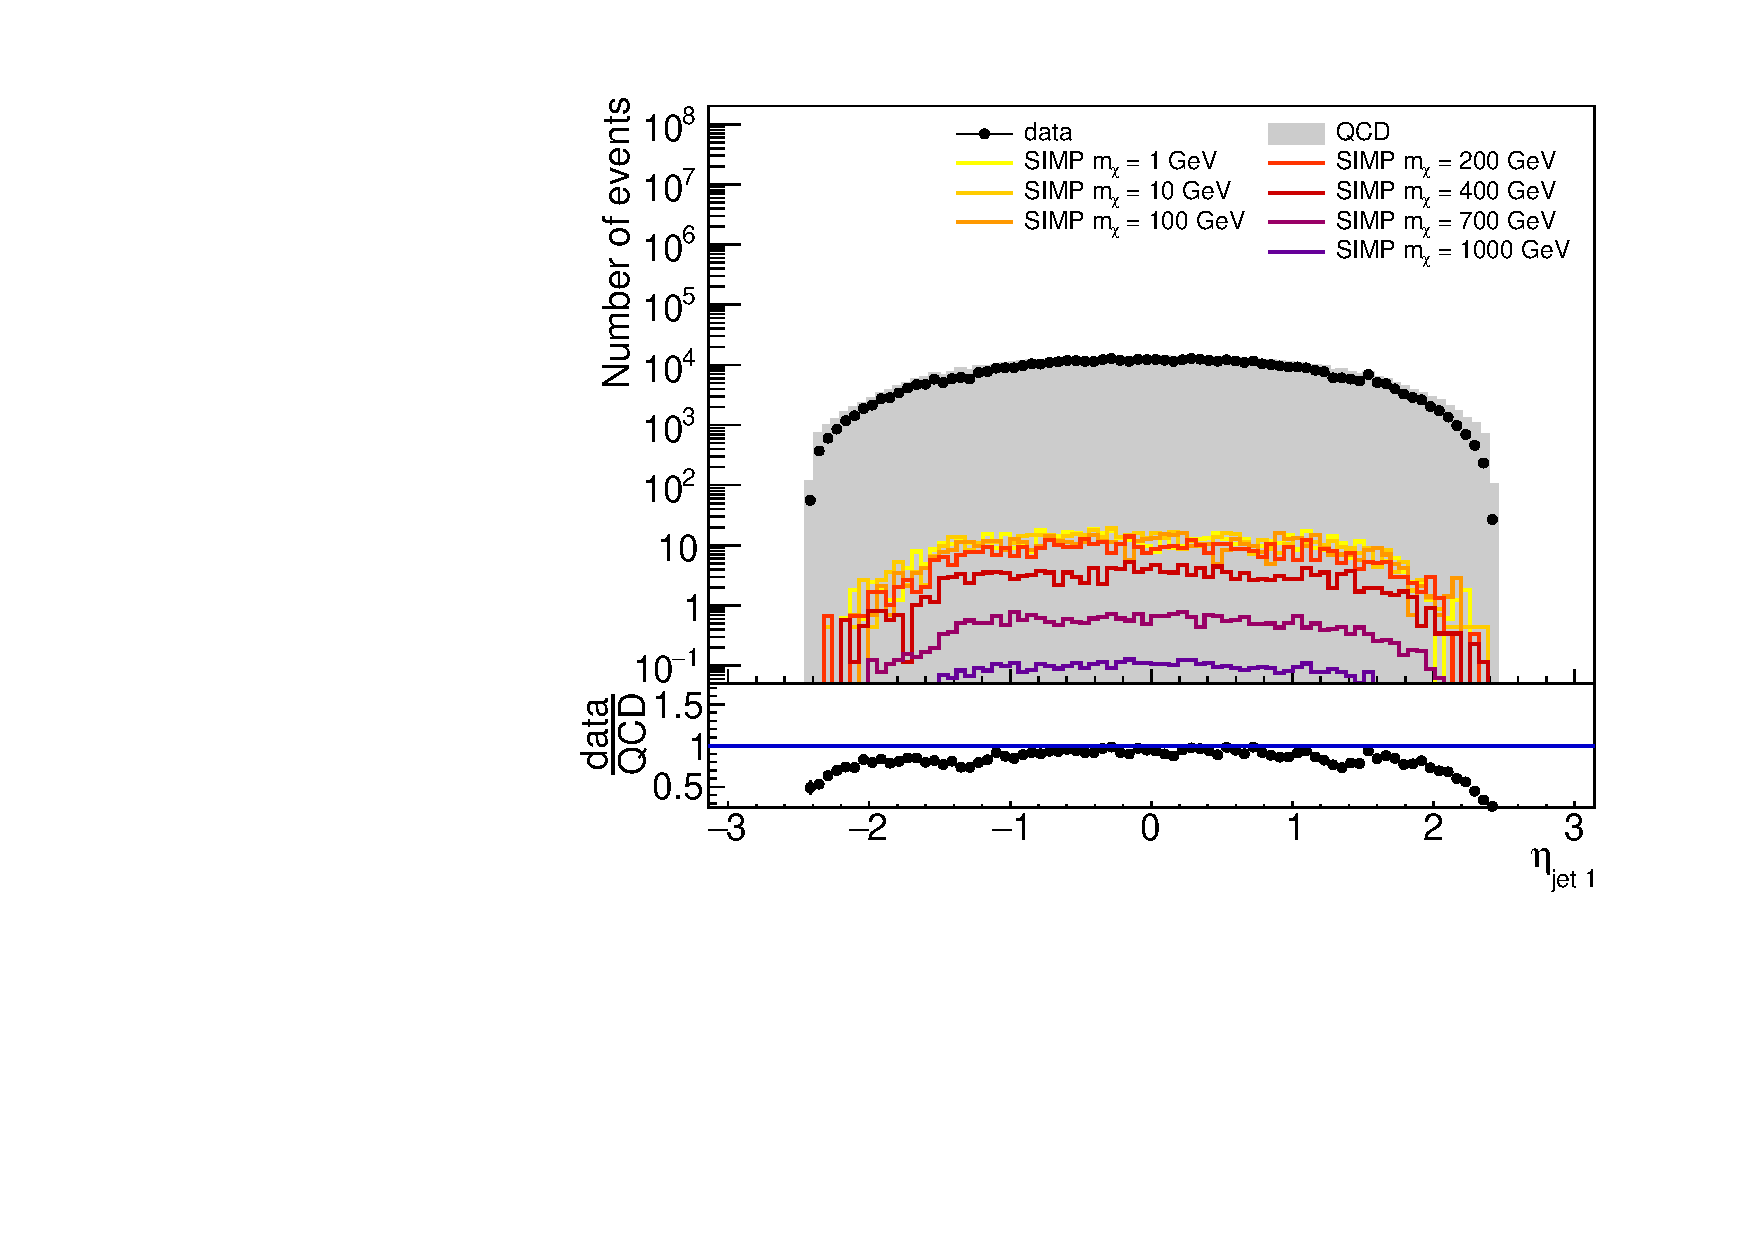
\includegraphics[width=0.5\textwidth]{figures/jet1_eta_newtrigger}\hfill%
  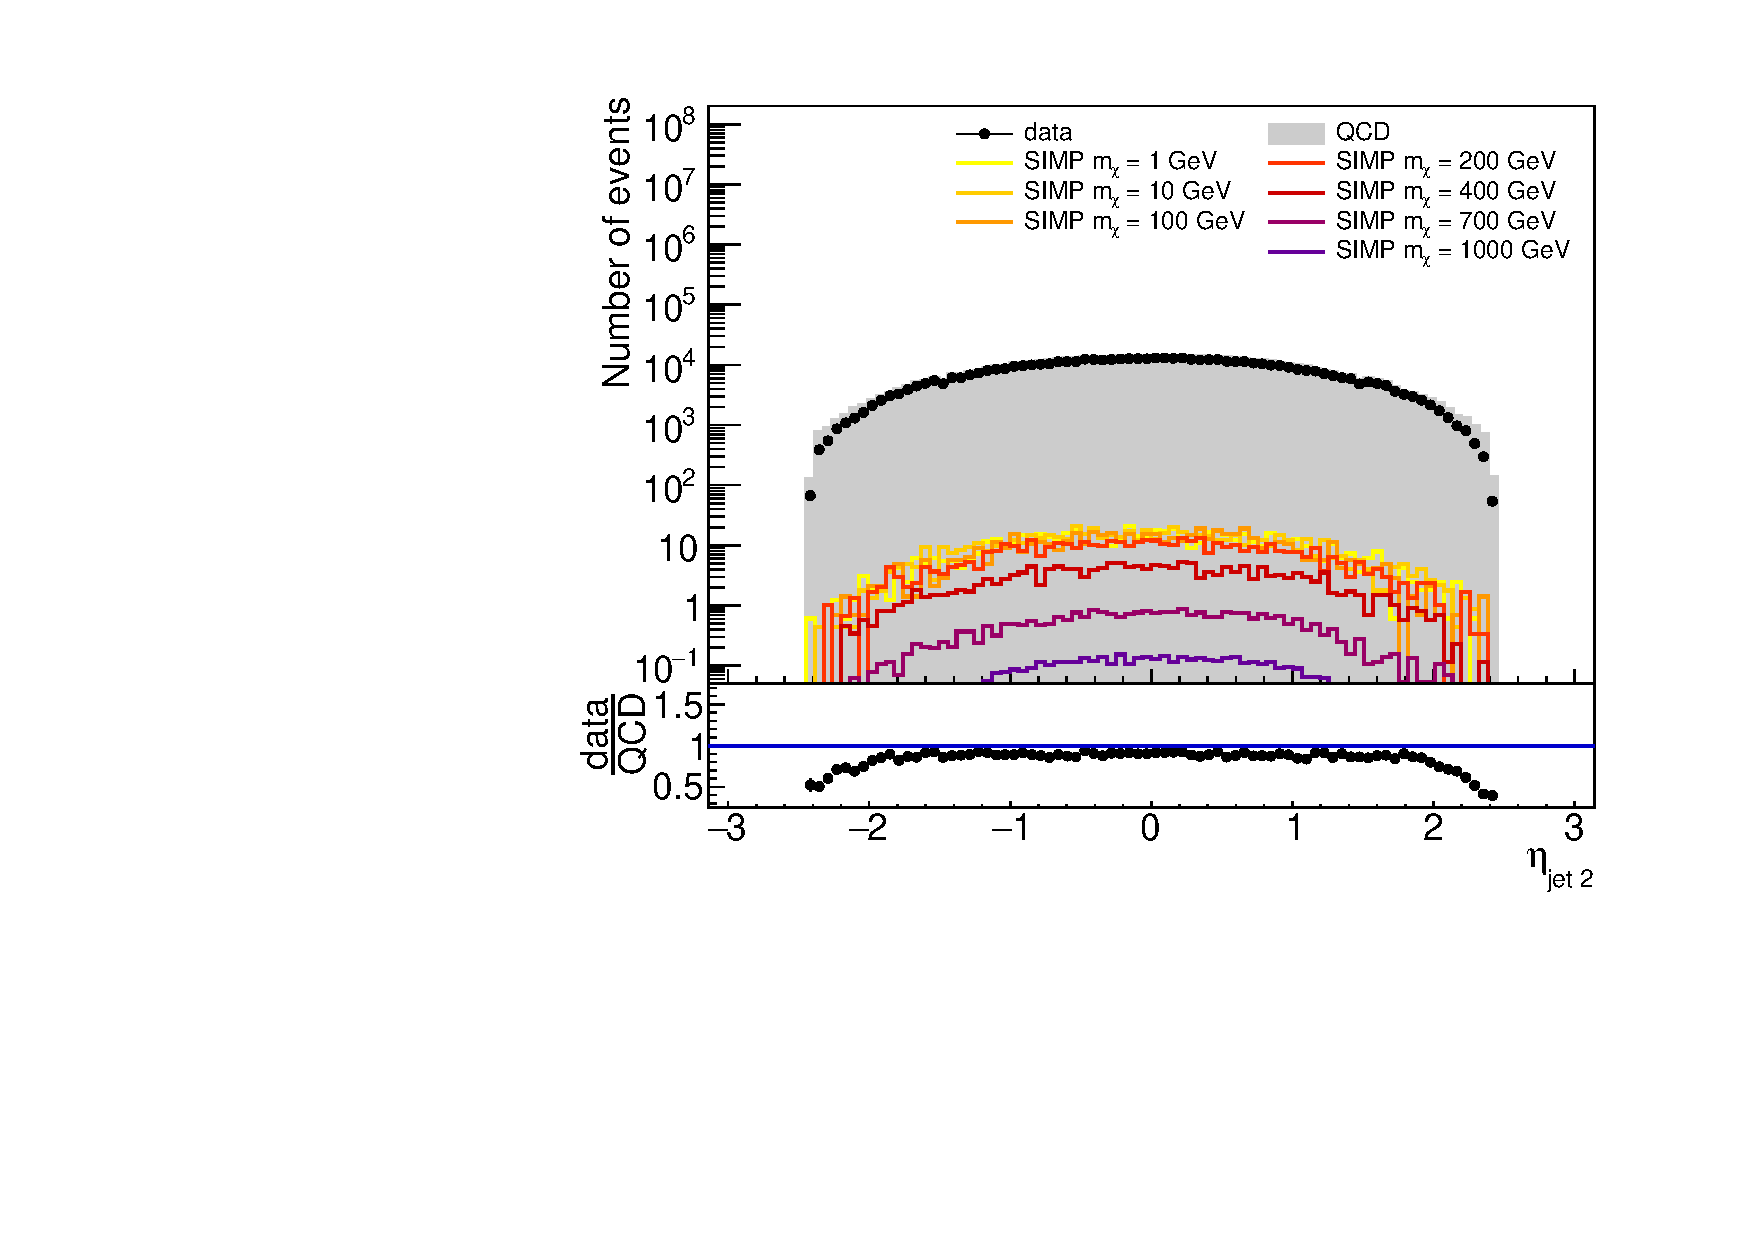
\includegraphics[width=0.5\textwidth]{figures/jet2_eta_newtrigger}
  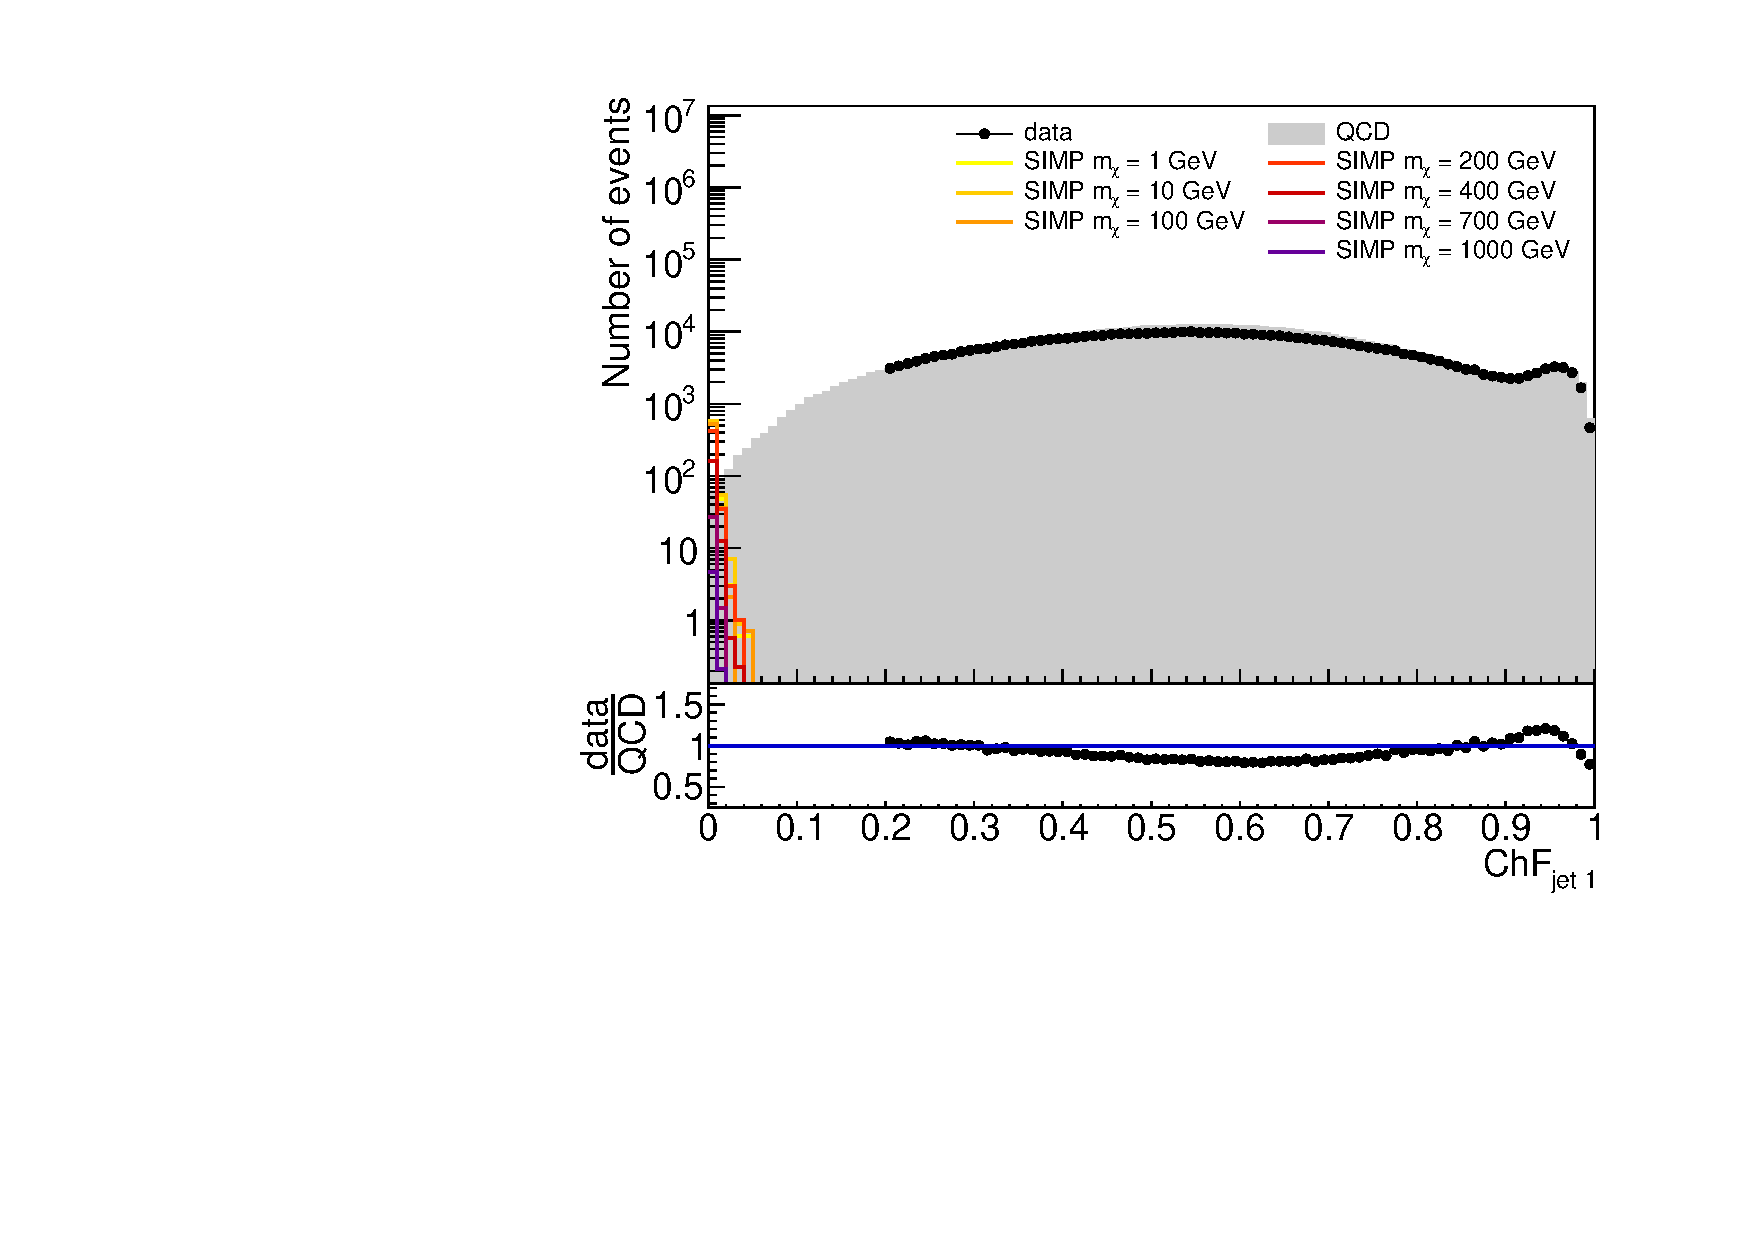
\includegraphics[width=0.5\textwidth]{figures/jet1_chf_newtrigger}\hfill%
  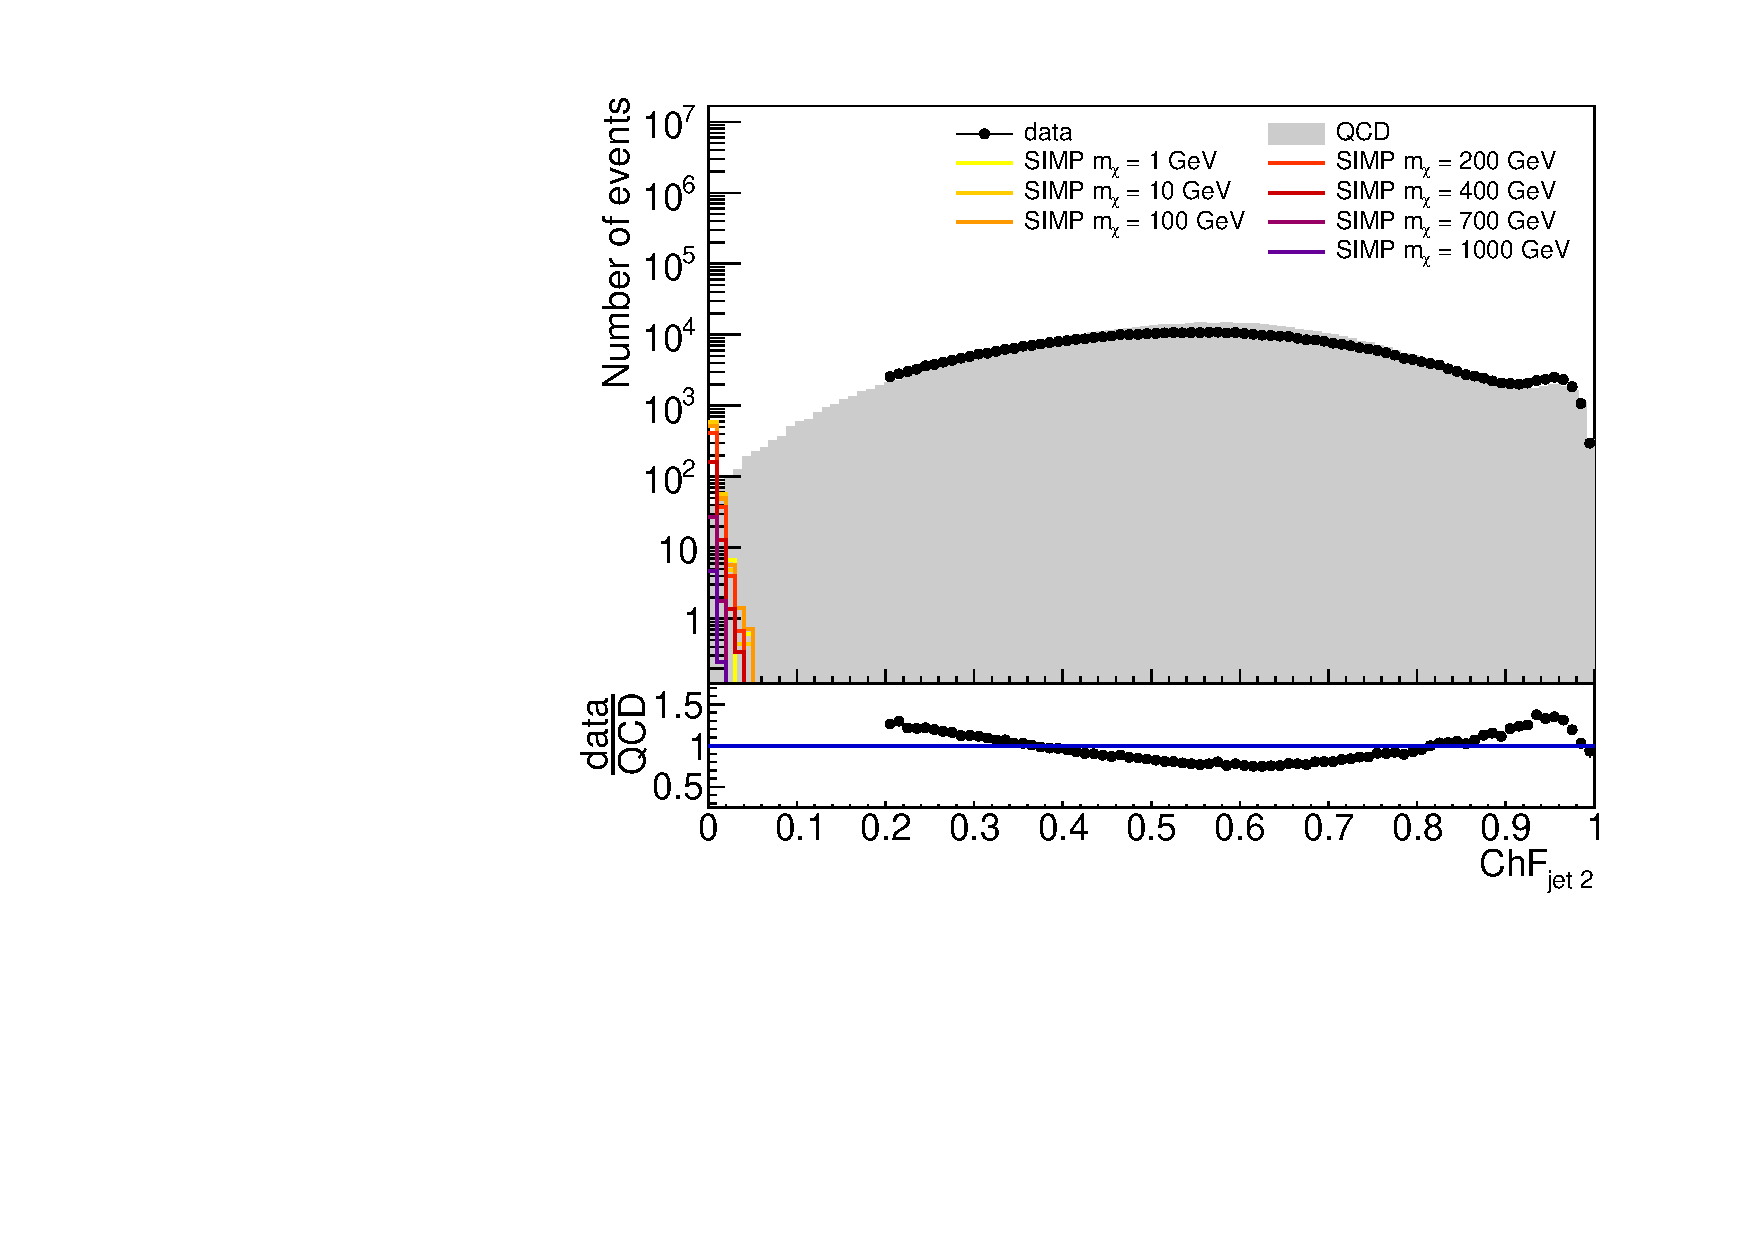
\includegraphics[width=0.5\textwidth]{figures/jet2_chf_newtrigger}
  \caption{$p_T$, $\eta$ and CHF of the leading (left) and subleading (right) jet. The selection cuts are applied, except for the cut on $\eta$ in the corresponding plot.}
  \label{fig:event_selection}
\end{figure}

As will be detailed in Section~\ref{sec:SIMP_backgrounds}, the background is predicted from a data control region where at least one of the leading jets has a high CHF, above $0.25$. No further selection on the second reconstruction with respect to the second primary vertex is applied for the control region, since the presence of at least one jet with a large CHF avoids the problem of the wrong selection of primary vertex detailed in Section~\ref{sec:SIMP_reconstruction}.

In the case of the signal region selection, both jets are required to have CHF $< x$, where $x$ is the signal cut being considered. In this case, the cut is applied for both reconstructions starting from the first and second primary vertex.

\section{Background estimation}
\label{sec:SIMP_backgrounds}

The main background for this analysis is \ac{QCD} multijets. This background is estimated from data, as the simulation does not describe the data well, especially at low CHF. The signal events can then be distinguished from this background using the jet CHF. A second background comes from photon + jets events. However, this background is efficiently removed by applying a photon veto.

\subsection{Photon + jets}

The photon + jets background was studied using a high-$H_T$ MC sample generated at \ac{LO} with \textsc{MadGraph5\_}a\textsc{MC@NLO}, hadronized with \textsc{Pythia 8}, and simulated and reconstructed using the standard procedure described in Chapter~\ref{ch:reconstruction}. The used sample corresponds to about $27\, \mathrm{fb}^{-1}$, which is larger than the data sample used for this analysis and was found to be sufficient to evaluate its contribution in the signal region. This background is verified to be negligible after applying the signal region event selection, and well within any other systematic uncertainty on the background prediction. The photon veto works well, especially the cut on the jet neutral electromagnetic fraction, and no events from the used simulated photon + jets sample remain after applying a cut of CHF $<$ 0.1. Additionally, in part of the events remaining just above that cut the photon is not identified because it is very close to a jet. These events are therefore already contained in the overlapping \ac{QCD} multijets sample.

\subsection{QCD multijets}

The \ac{QCD} multijet background is estimated from data, since the simulation does not describe the data well, especially at low CHF, as can be seen from Figure~\ref{fig:dataMC} which compares the CHF distribution in the control region to the \ac{QCD} MC. In this plot the subleading jet is required to have a large CHF, in order to stay in the control region.

\begin{figure}[ht]
  \centering
  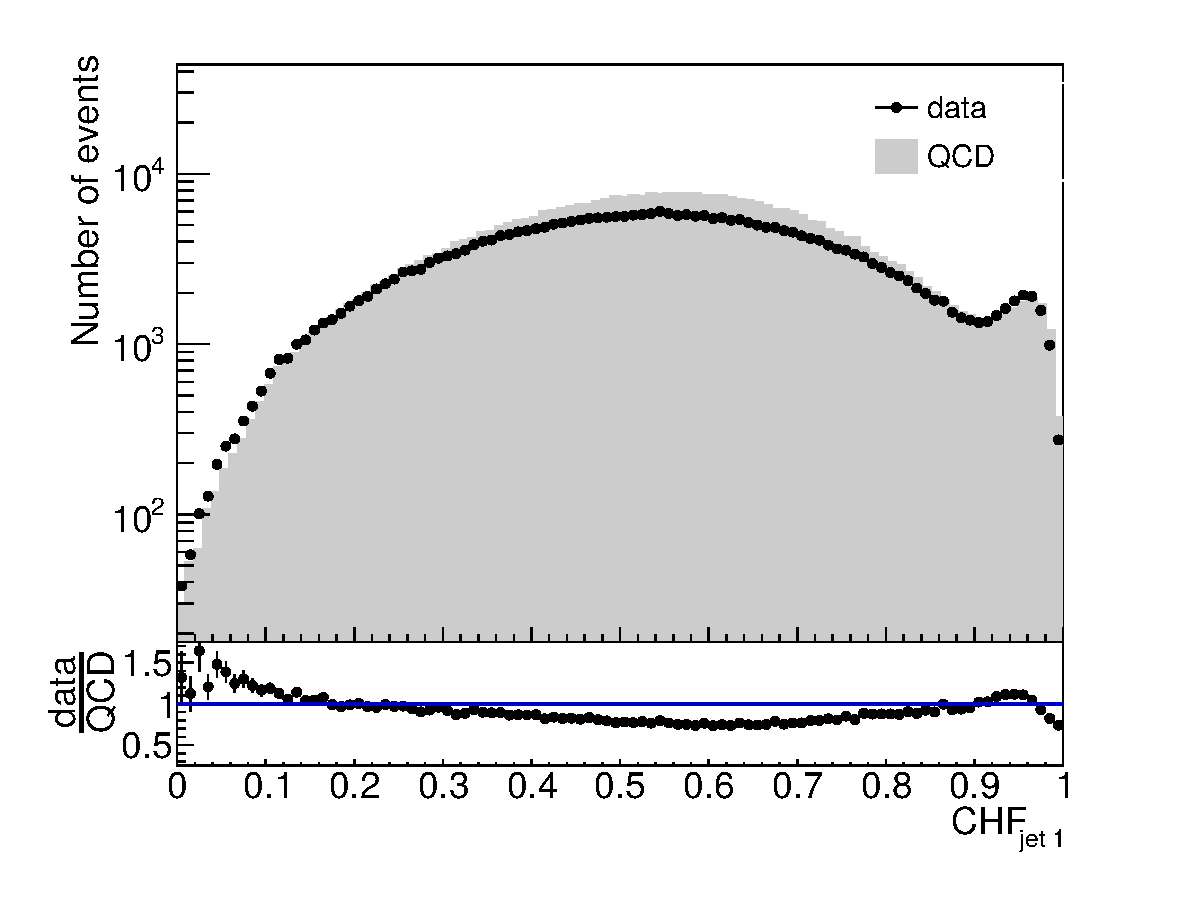
\includegraphics[width=0.7\textwidth]{figures/bkgd_estimation_dataMC.pdf}\hfill%
  \caption{Data-MC comparison of the charged energy fraction of the leading jet, tagging events with subleading jet CHF $>$ 0.5.}
  \label{fig:dataMC}
\end{figure}

As a first step, the efficiency of the CHF cut is measured in the control region, by tagging one jet with high CHF and applying the CHF cut on the other jet. The efficiency is then given by the ratio of the number of events passing the cut divided by the total number of events selected in the control region. The measurement is performed in bins of jet $p_T$ and $\eta$. The number of \ac{QCD} events in the signal region is then predicted by using any \ac{QCD} dijet event passing the selection cuts listed in Table~\ref{tab:cutflow} and applying the appropriate $p_T$ and $\eta$ dependent CHF cut efficiencies on the two leading jets. Figure~\ref{fig:efficiencies} shows the measured efficiency as a function of the CHF cut for various bins in $p_T^{jet}$, integrating over the $\eta_{jet}$ bins, and $\eta_{jet}$, integrating of the $p_T^{jet}$ bins, as measured in the \ac{QCD} MC. There is a strong dependence on the jet $p_T$, and a less pronounced dependence on the jet $\eta$ at low CHF. The efficiencies are the highest for the $1.0 < |\eta| < 1.25$ bin, which can be attributed to this being the barrel-endcap transition region where most of the tracker material is located. The dependence on the jet $p_T$ arises from the reconstruction. As can be seen from the left plot in Figure~\ref{fig:pt_dependence}, at generator level the CHF is independent of the jet $p_T$, as one would expect. After reconstruction, as demonstrated in the right plot of Figure~\ref{fig:pt_dependence}, a $p_T$ dependence arises due to the known degradation of tracking efficiency in dense jet environments, which becomes more of an issue for very high $p_T$ and thus collimated jets.

\begin{figure}[ht]
  \centering
  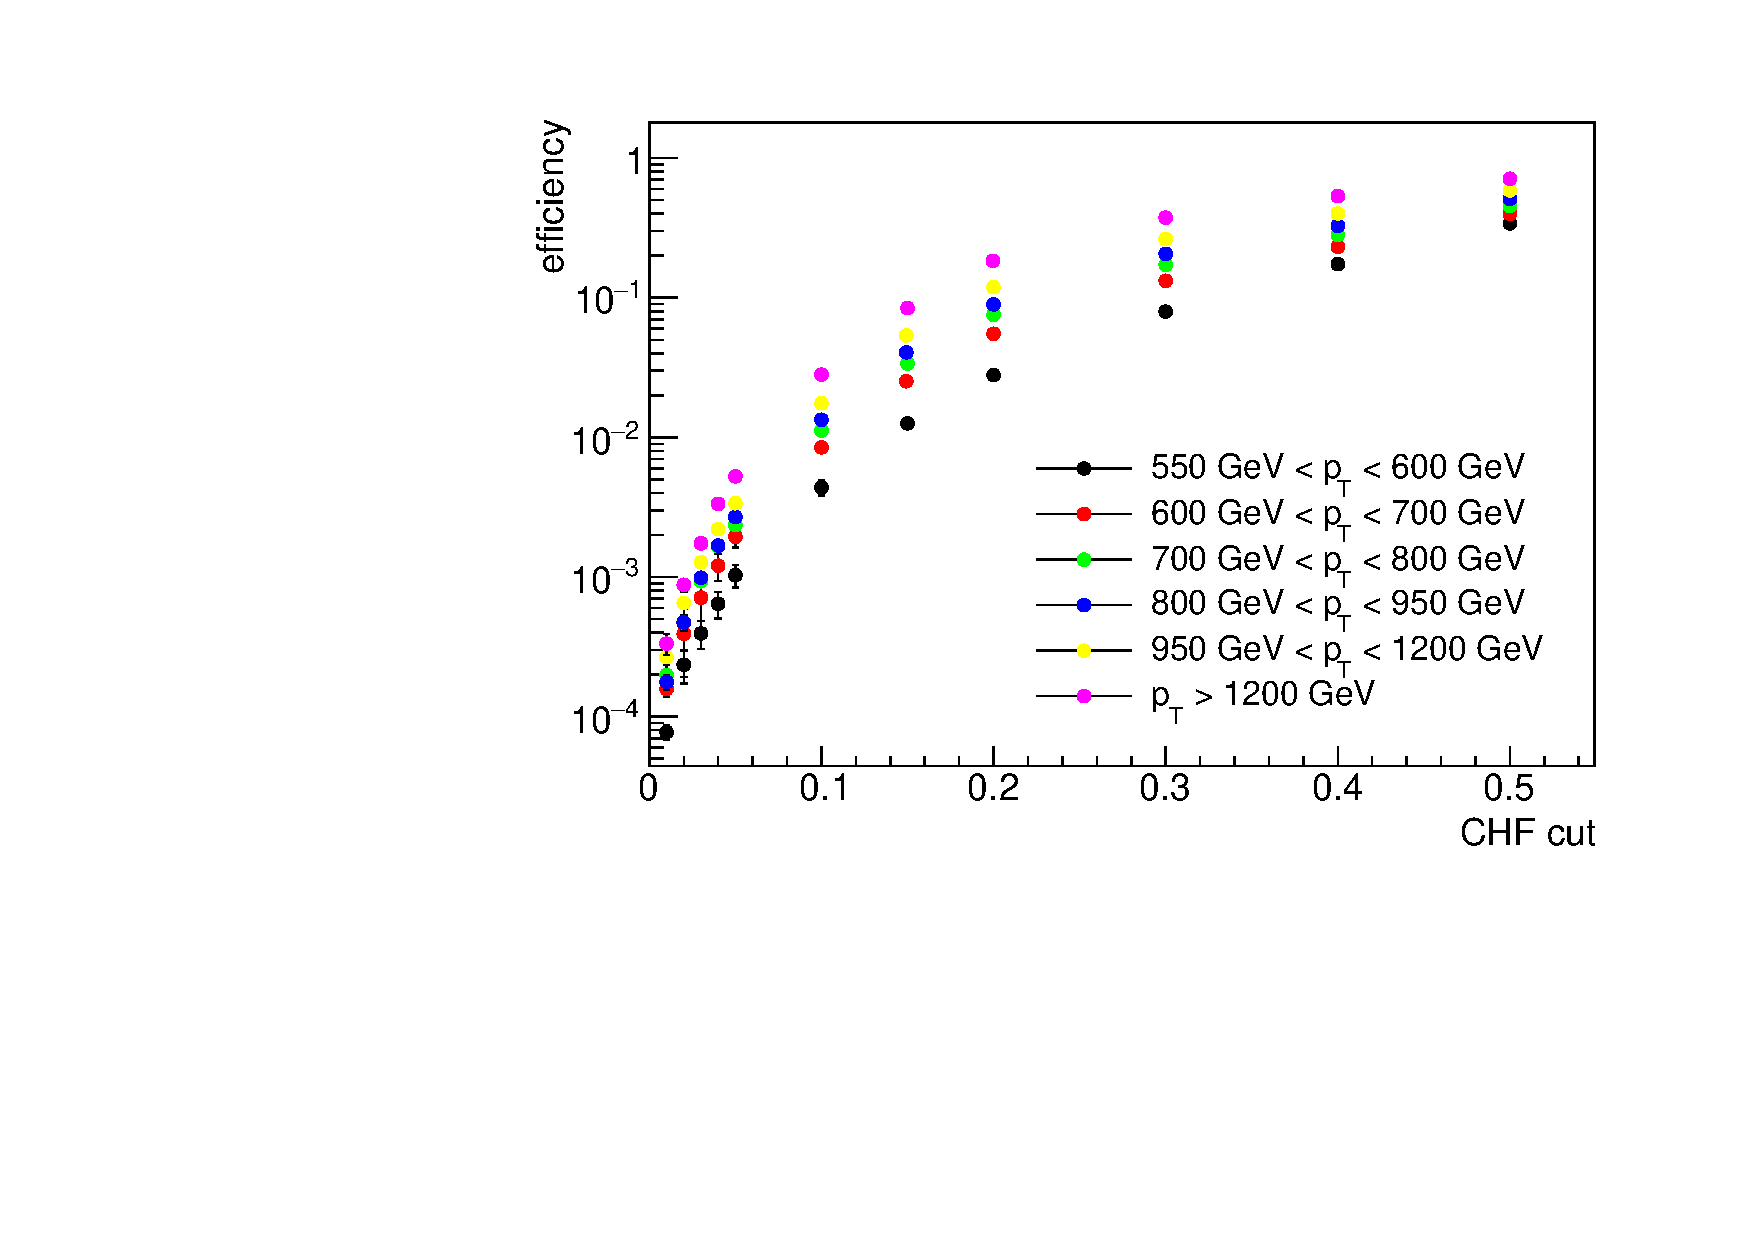
\includegraphics[width=0.5\textwidth]{figures/eff1D_pt_newtrigger.pdf}\hfill%
  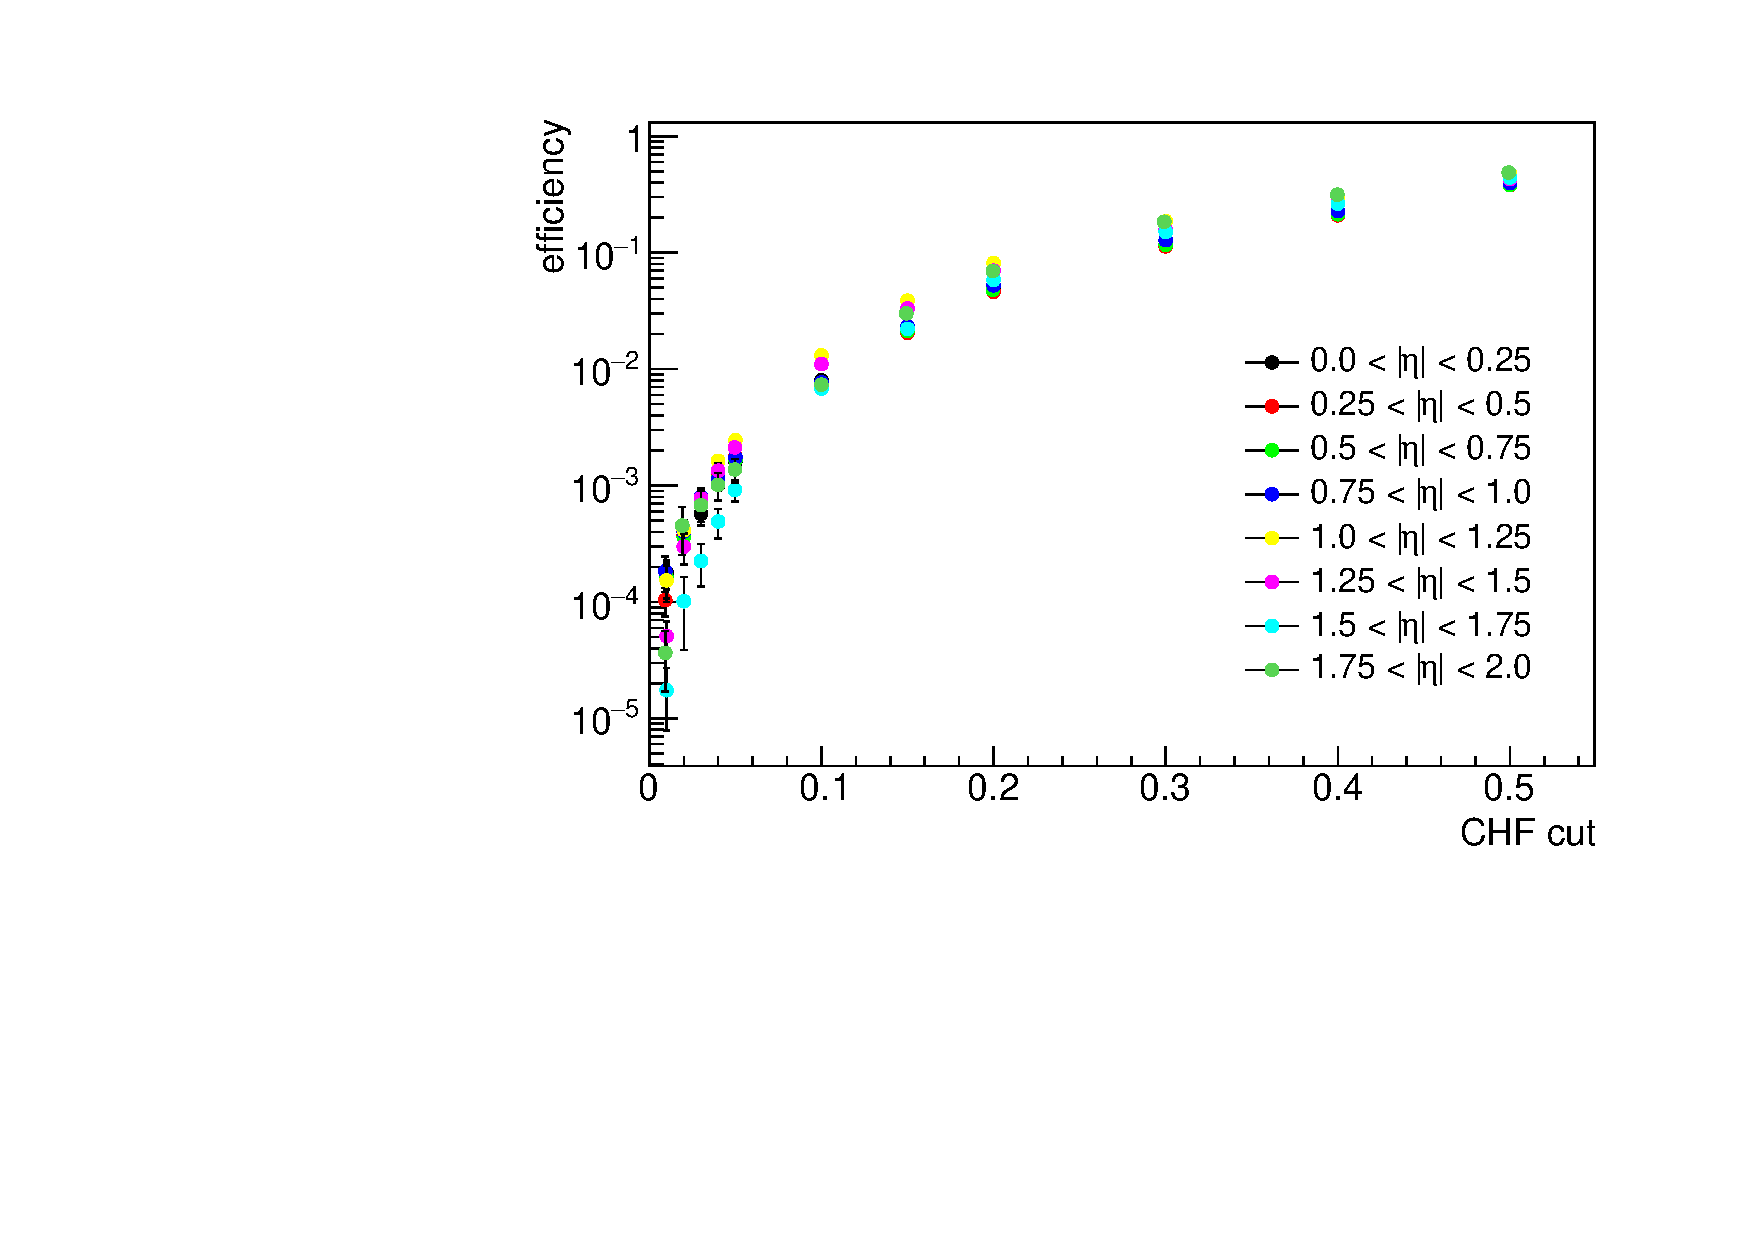
\includegraphics[width=0.5\textwidth]{figures/eff1D_eta_newtrigger.pdf}
  \caption{The efficiency of several CHF cuts in \ac{QCD} MC, binned in $p_T$ (left) and $\eta$ (right).}
  \label{fig:efficiencies}
\end{figure}

\begin{figure}[ht]
  \centering
  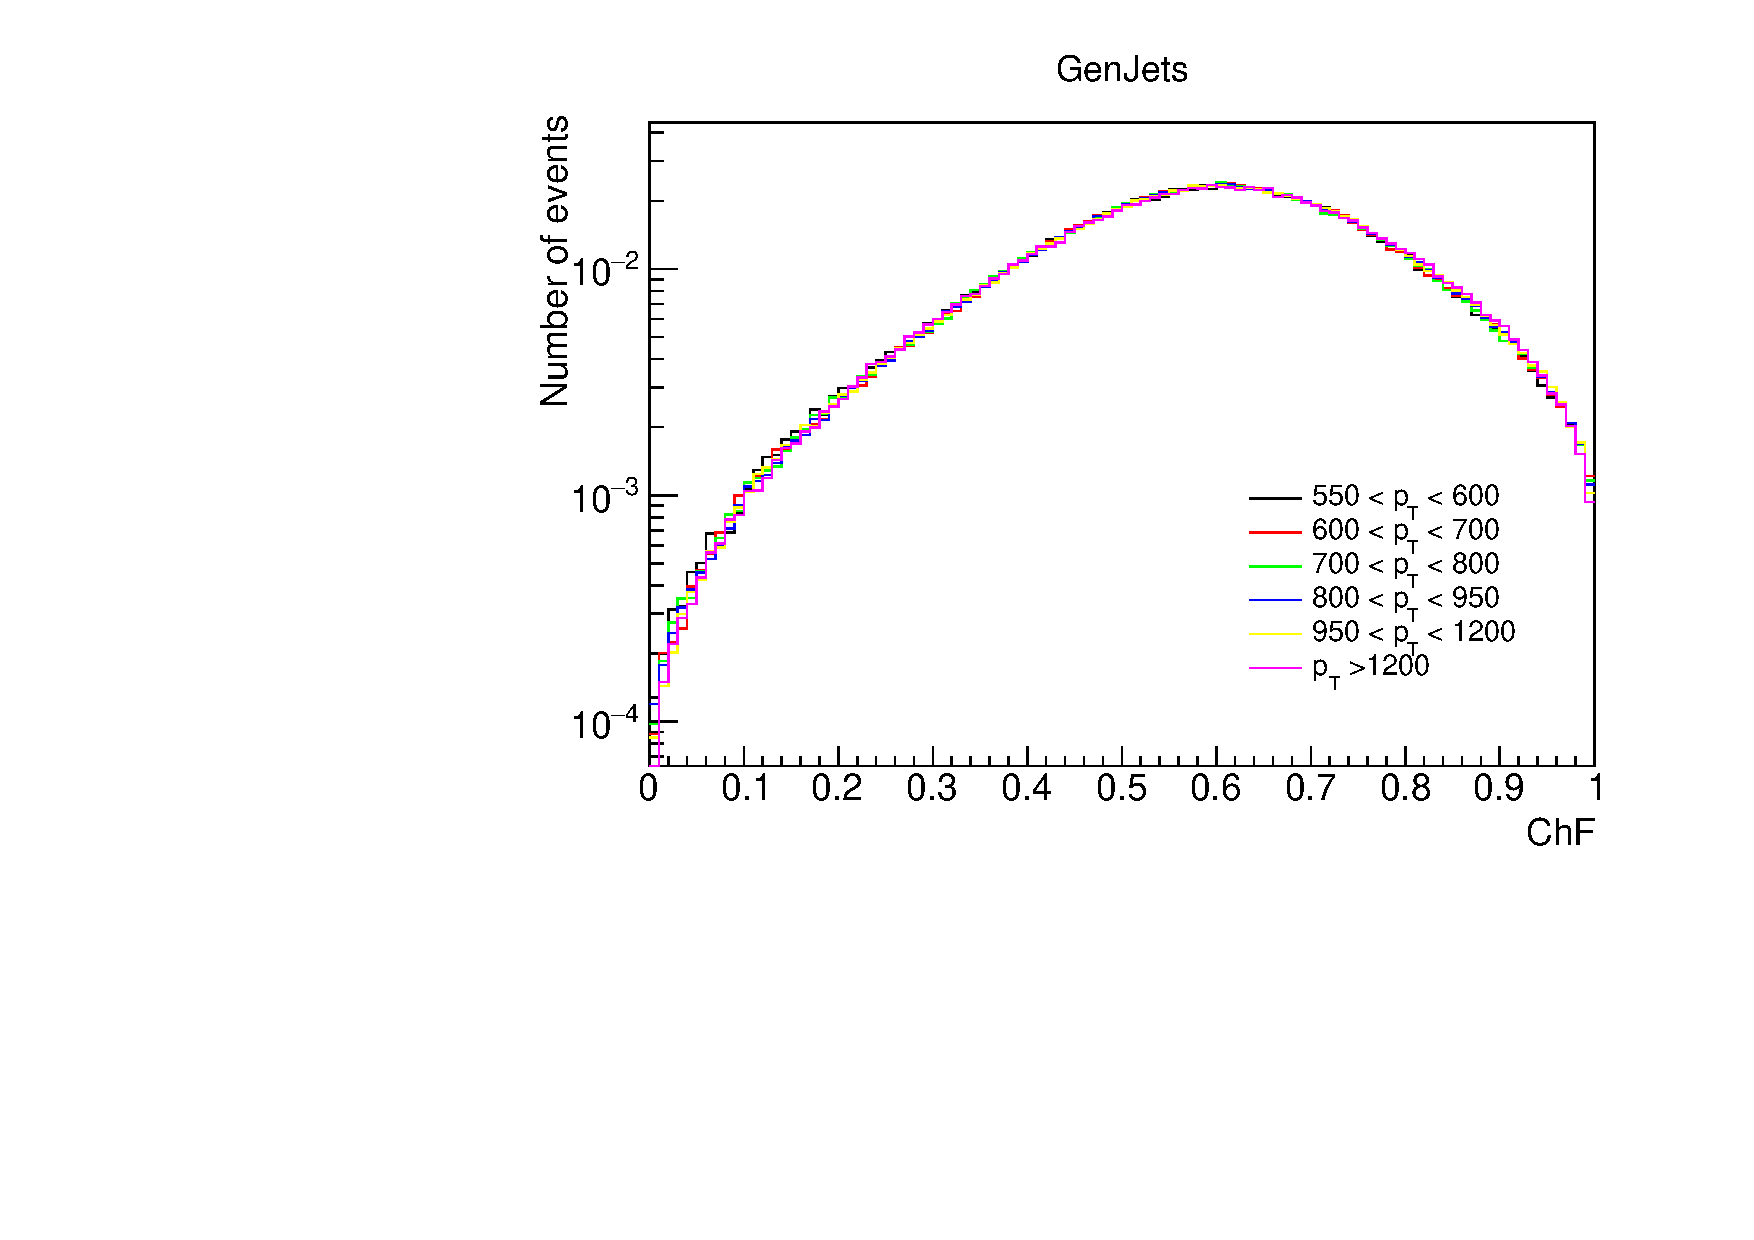
\includegraphics[width=0.5\textwidth]{figures/ChFPerPtbin_GenJets.pdf}\hfill%
  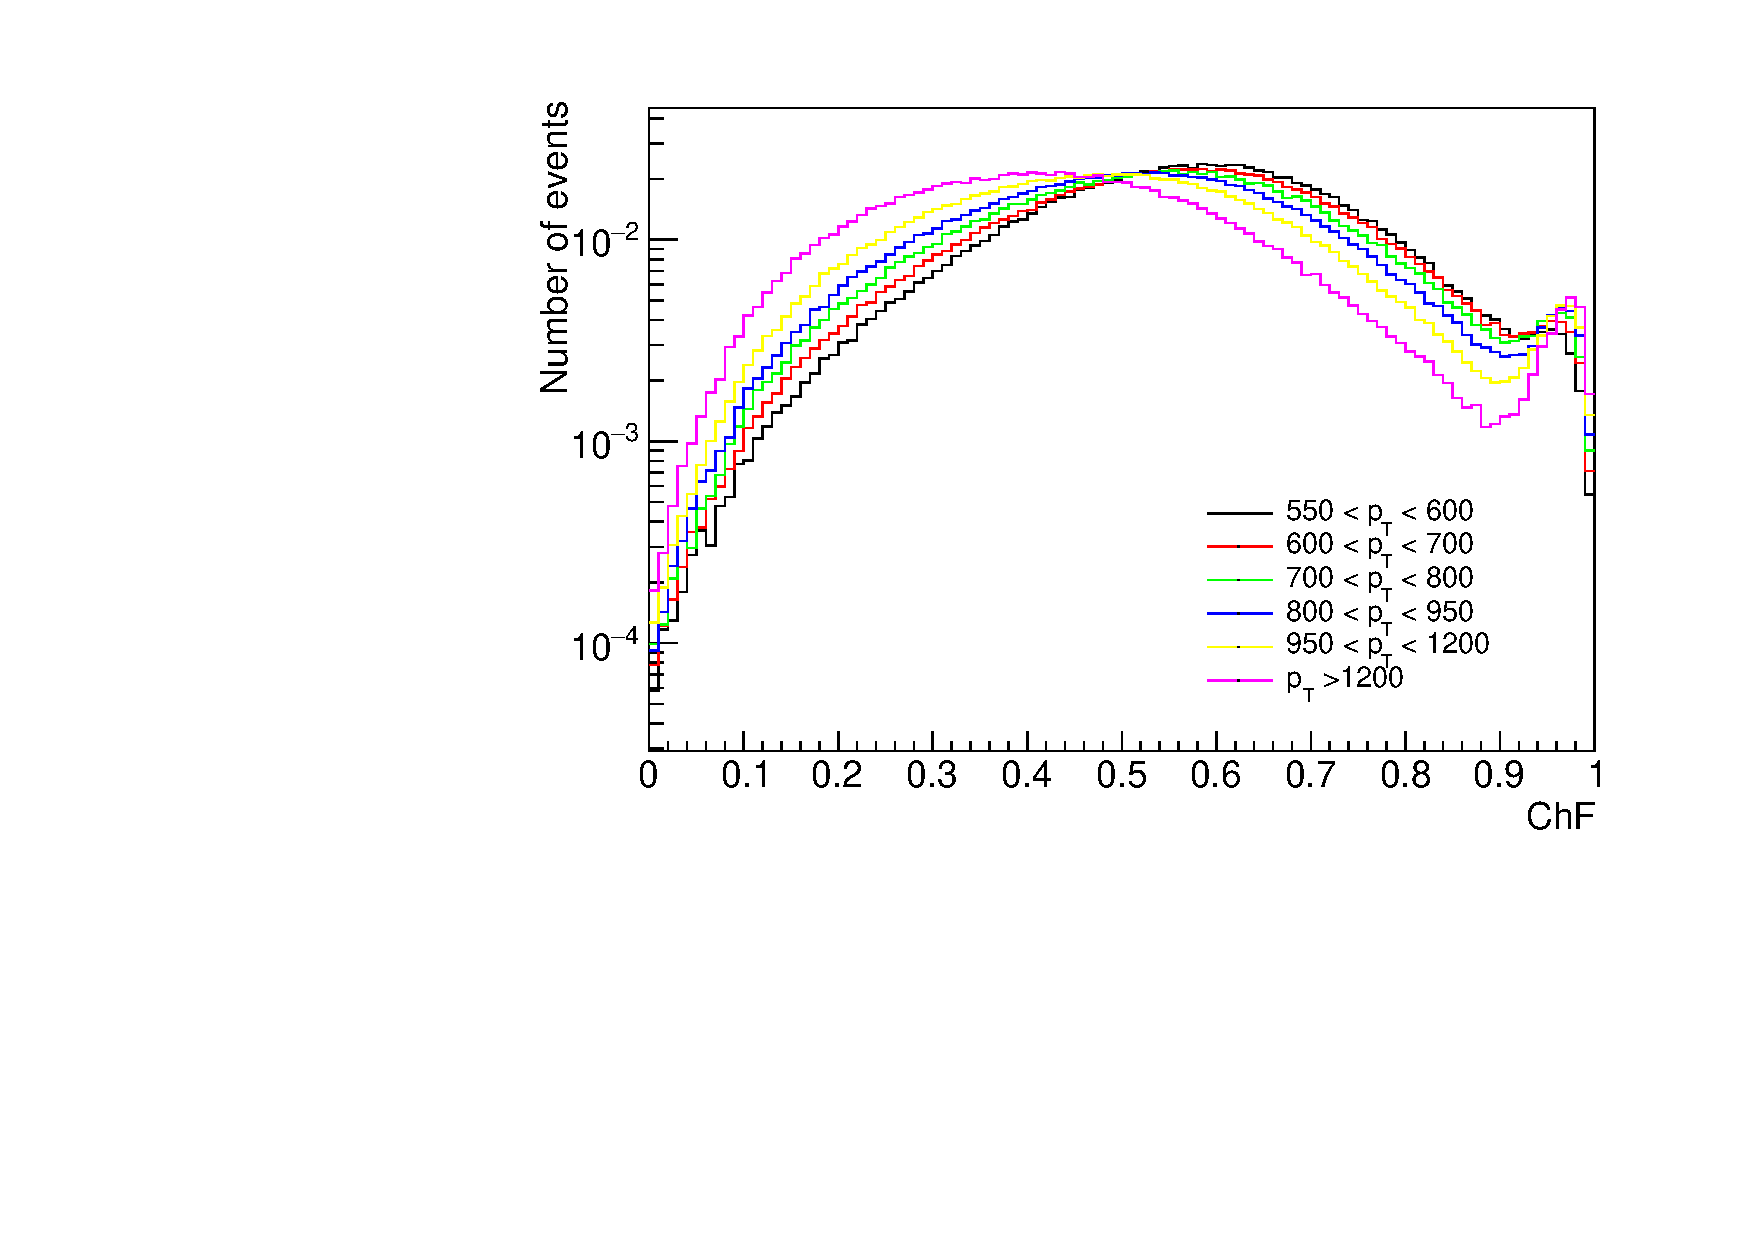
\includegraphics[width=0.5\textwidth]{figures/ChFperPtbin.pdf}
  \caption{The CHF per bins of jet $p_T$, for generator level (left) and reconstructed (right) jets.}
  \label{fig:pt_dependence}
\end{figure}

A test of the background prediction method is performed using simulated events in order to validate it. This is done by comparing the MC truth and the so-called 1- and 2-leg predictions. The MC truth shows the yield after applying the CHF cuts on both jets. For the 1-leg prediction the CHF cut is applied on one jet and the event is then weighted by applying the measured $p_T$- and $\eta$-dependent efficiency for the other jet. For the 2-leg prediction, the efficiencies are applied for both jets, and no CHF cut is applied directly.

As a first check, the test was also performed at the generator level, using the GenJets, which are reconstructed from the generator level particles. This comparison is done in exclusive bins in (CHF$_{\mathrm{jet 1}}$, CHF$_{\mathrm{jet 2}}$), as illustrated in Figure~\ref{fig:excl_binning}. From Figure~\ref{fig:closuretest_GenJets} one can see that there is a good agreement between MC truth, 1-, and 2-leg predictions. This shows that there are no relevant physics correlations between the 2 jets, an essential prerequisite for this background prediction to work well, and proves the $p_T$ and $\eta$ binning is adequate as well.

\begin{figure}[ht]
  \centering
  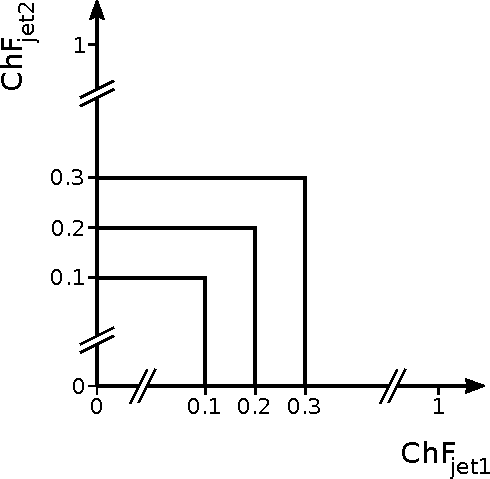
\includegraphics[width=0.45\textwidth]{figures/exclusive_binning.pdf}\hfill%
  \caption{Illustration of the exclusive bins in the leading and subleading jet CHF, used for test of the background prediction method and the data vs. prediction comparisons.}
  \label{fig:excl_binning}
\end{figure}

\begin{figure}[ht]
  \centering
  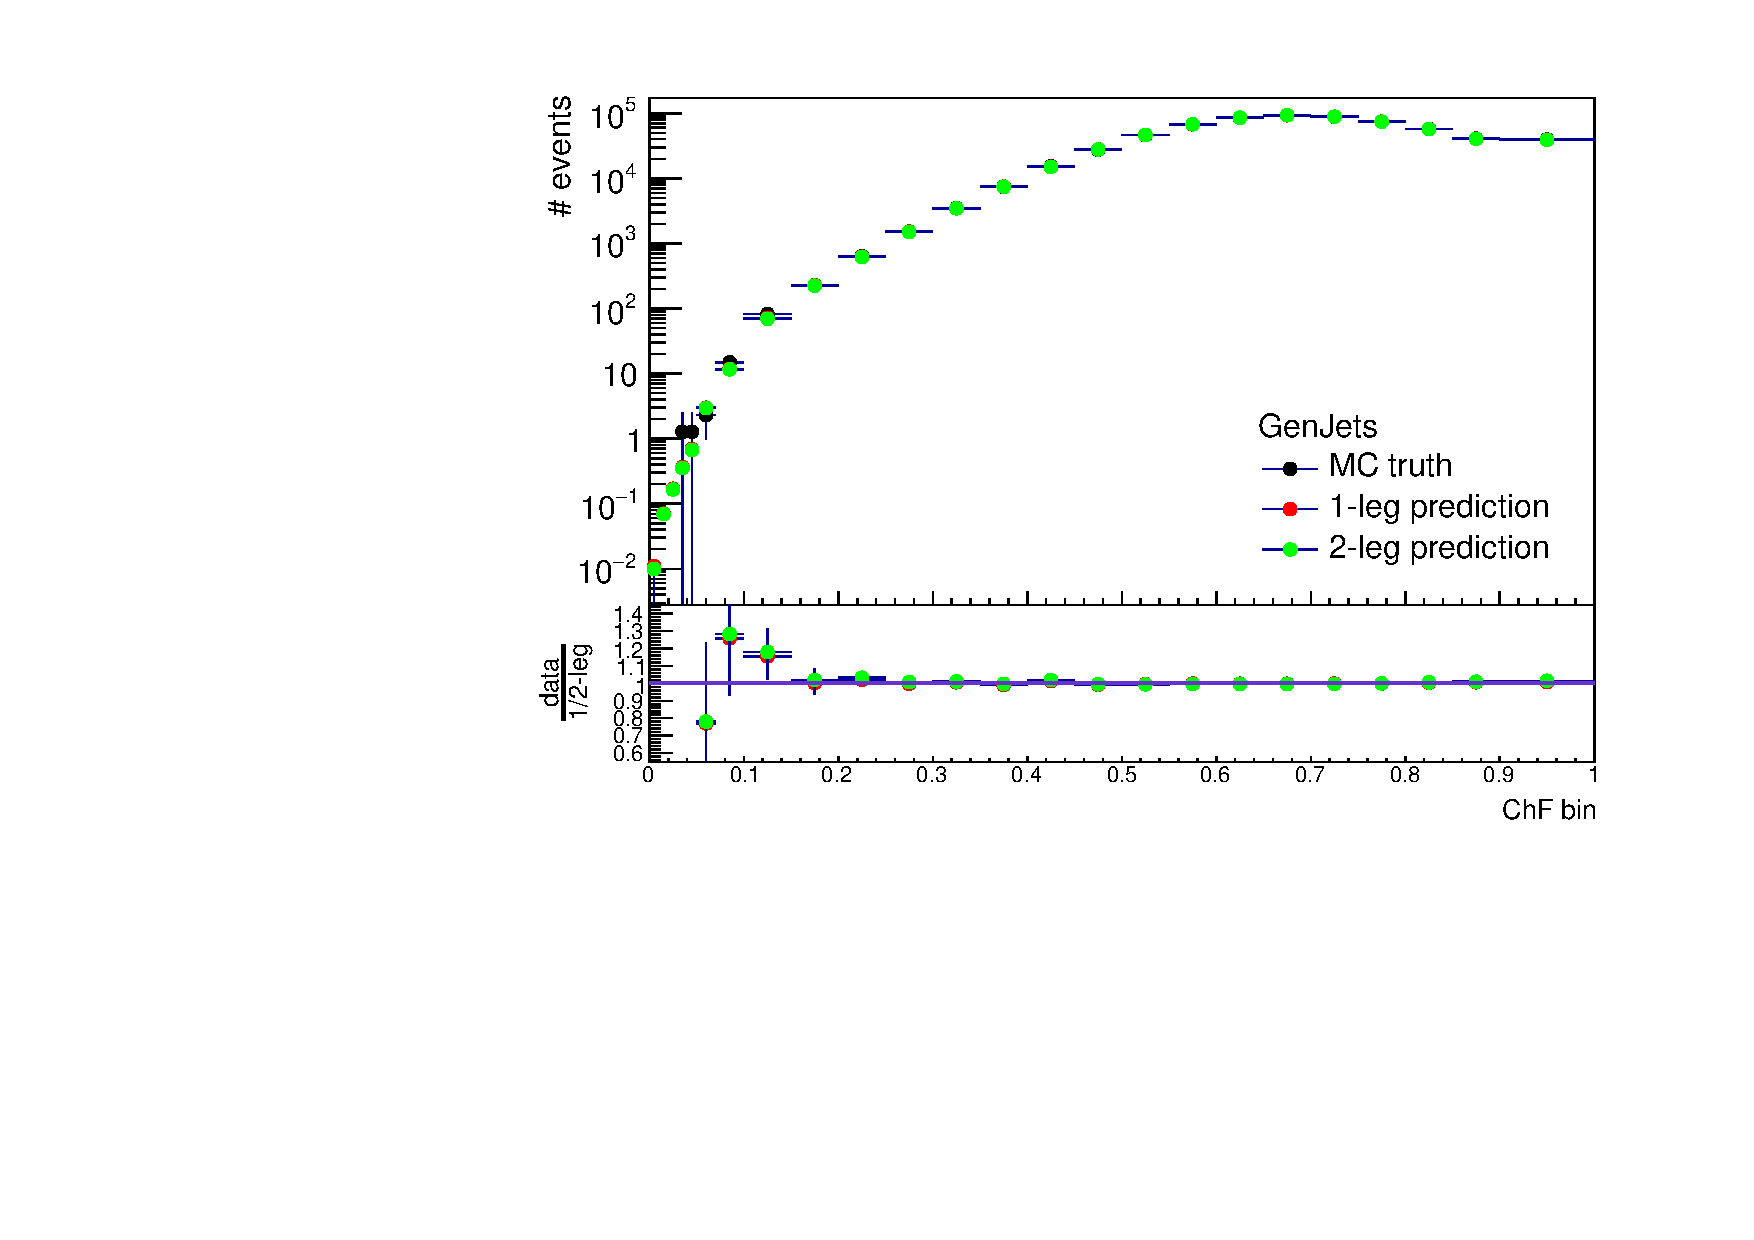
\includegraphics[width=0.75\textwidth]{figures/closure_test_QCD_GenJets_exclusive_correct.pdf}\hfill%
  \caption{Test of the background prediction method using the GenJets in simulated events. The number of events is scaled to $16.1\, \mathrm{fb}^{-1}$, corresponding to the amount of data used for this analysis.}
  \label{fig:closuretest_GenJets}
\end{figure}

Next, the test is performed with reconstructed jets, as shown in the left plot of Figure~\ref{fig:closuretest}, using the exclusive binning. For the MC truth, the CHF cut is applied on the 2 leading jets of the standard jet collection, as well as the 2 leading jets of the jet collection created when using the second vertex as primary vertex. This extra cut is a part of the signal region event selection described earlier, designed to remove events where the wrong primary vertex was chosen and the charged fraction of the jets is removed by \ac{CHS}. However, there is still a small discrepancy between the MC truth and the prediction at the tightest CHF cuts. This is mainly due to a very small number of events where the wrong vertex was chosen, but where the correct one is not the second one. The level of agreement reached is however already sufficient for the considered data sample.

The test of the method is also performed in inclusive bins, as used in the signal region event selection, by applying the same cut on the CHF of both jets. This is shown in the right plot of Figure~\ref{fig:closuretest}, with the applied CHF cut on the x-axis. For the MC truth, the statistical uncertainty is determined  per HT-binned \ac{QCD} sample, using asymmetric vertical bars with correct coverage for event counts with Poisson variates when less than 10 events remain, and the square root of the remaining number of events otherwise. In this way, the statistical uncertainty correctly reflects the contribution of HT bins with few or no events left. The total statistical uncertainty in the MC truth is then calculated by multiplying the uncertainty per HT bin by the corresponding weight for this HT bin, and adding them quadratically. The uncertainties on the 1- and 2-leg predictions are much smaller, as the statistical uncertainties from the efficiencies is negligible. The systematic uncertainty on the background prediction is then defined as the difference between the MC truth and the prediction, unless it is smaller than the statistical uncertainty on the MC truth. In that case, the uncertainty on the MC truth is taken as systematic uncertainty. For most CHF cut values, the statistical uncertainty dominates. As a result the background prediction is limited by the MC sample size.

\begin{figure}[ht]
  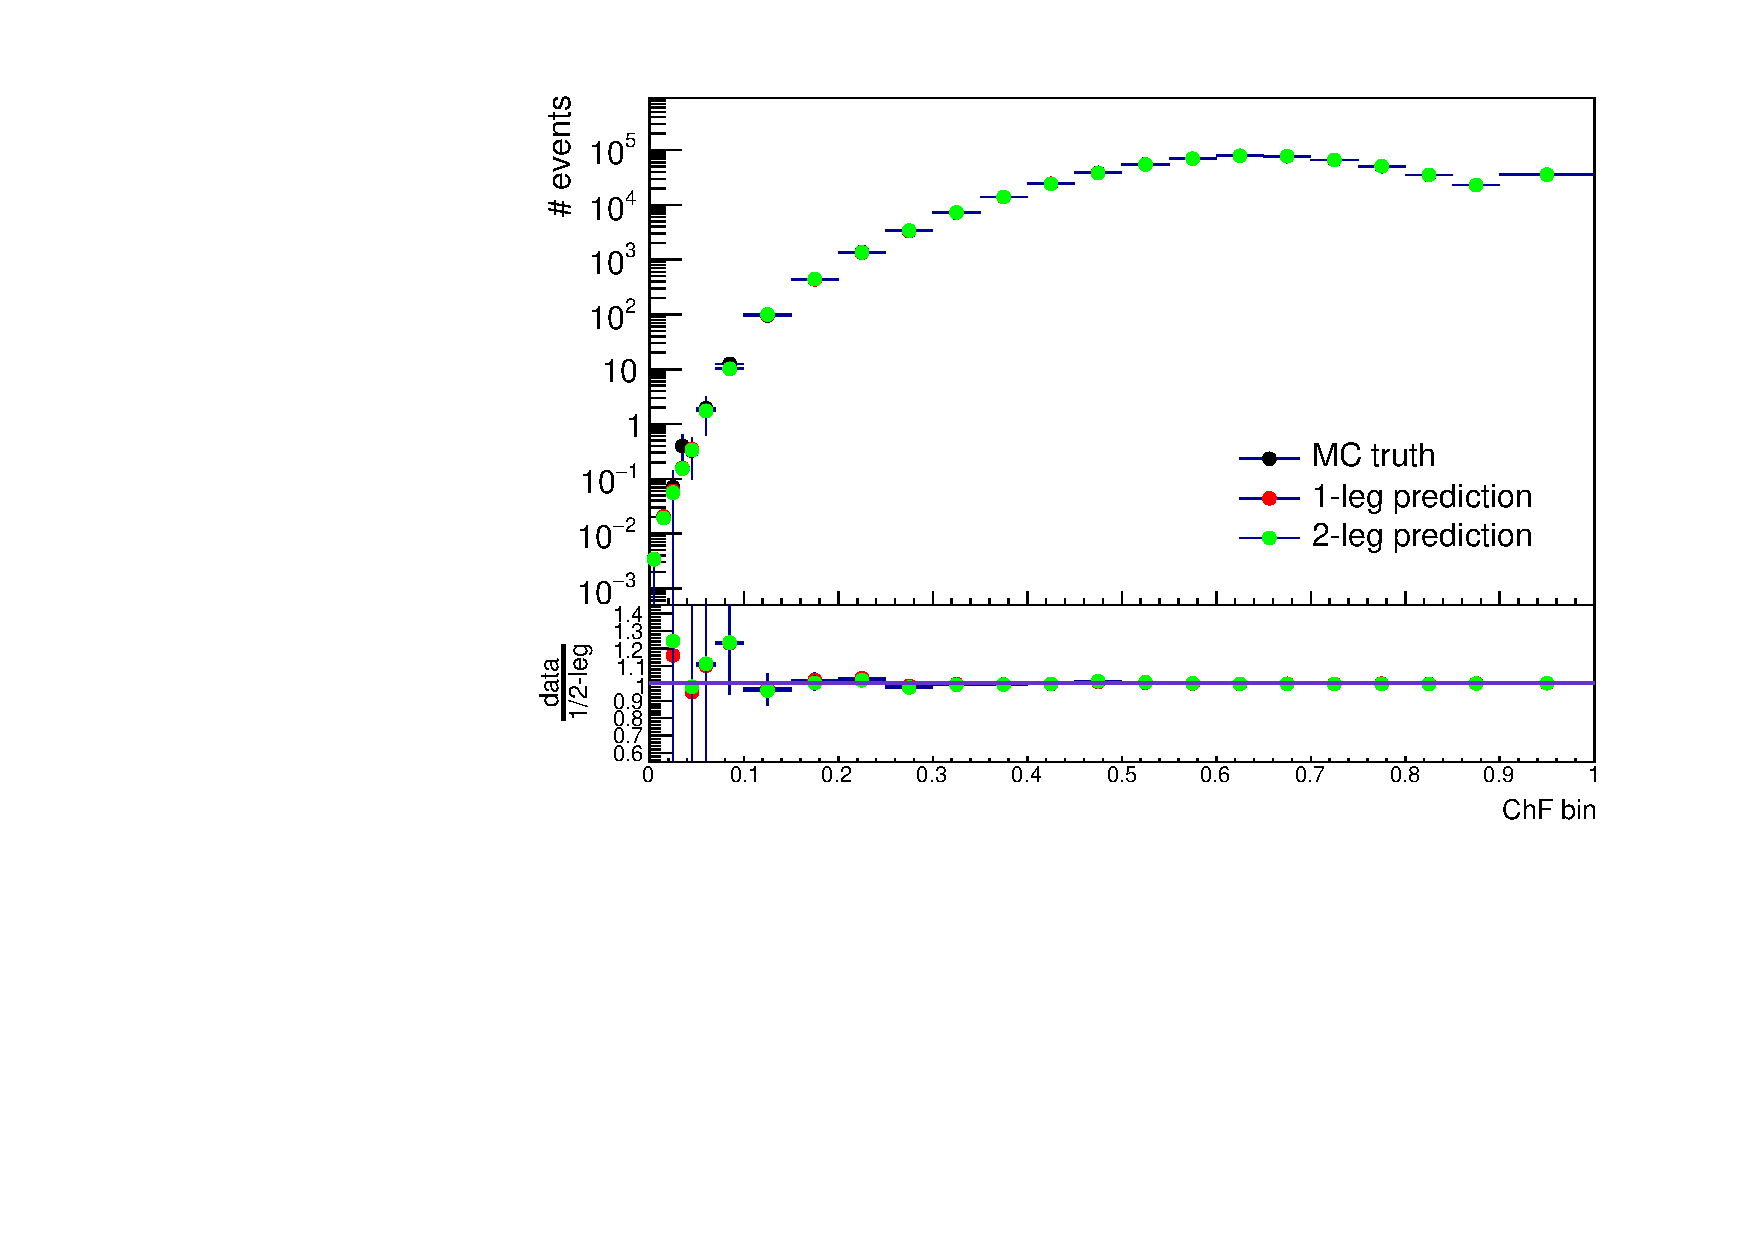
\includegraphics[width=0.52\textwidth]{figures/closure_test_QCD_exclusive_filters.pdf}\hspace{.2cm}%
  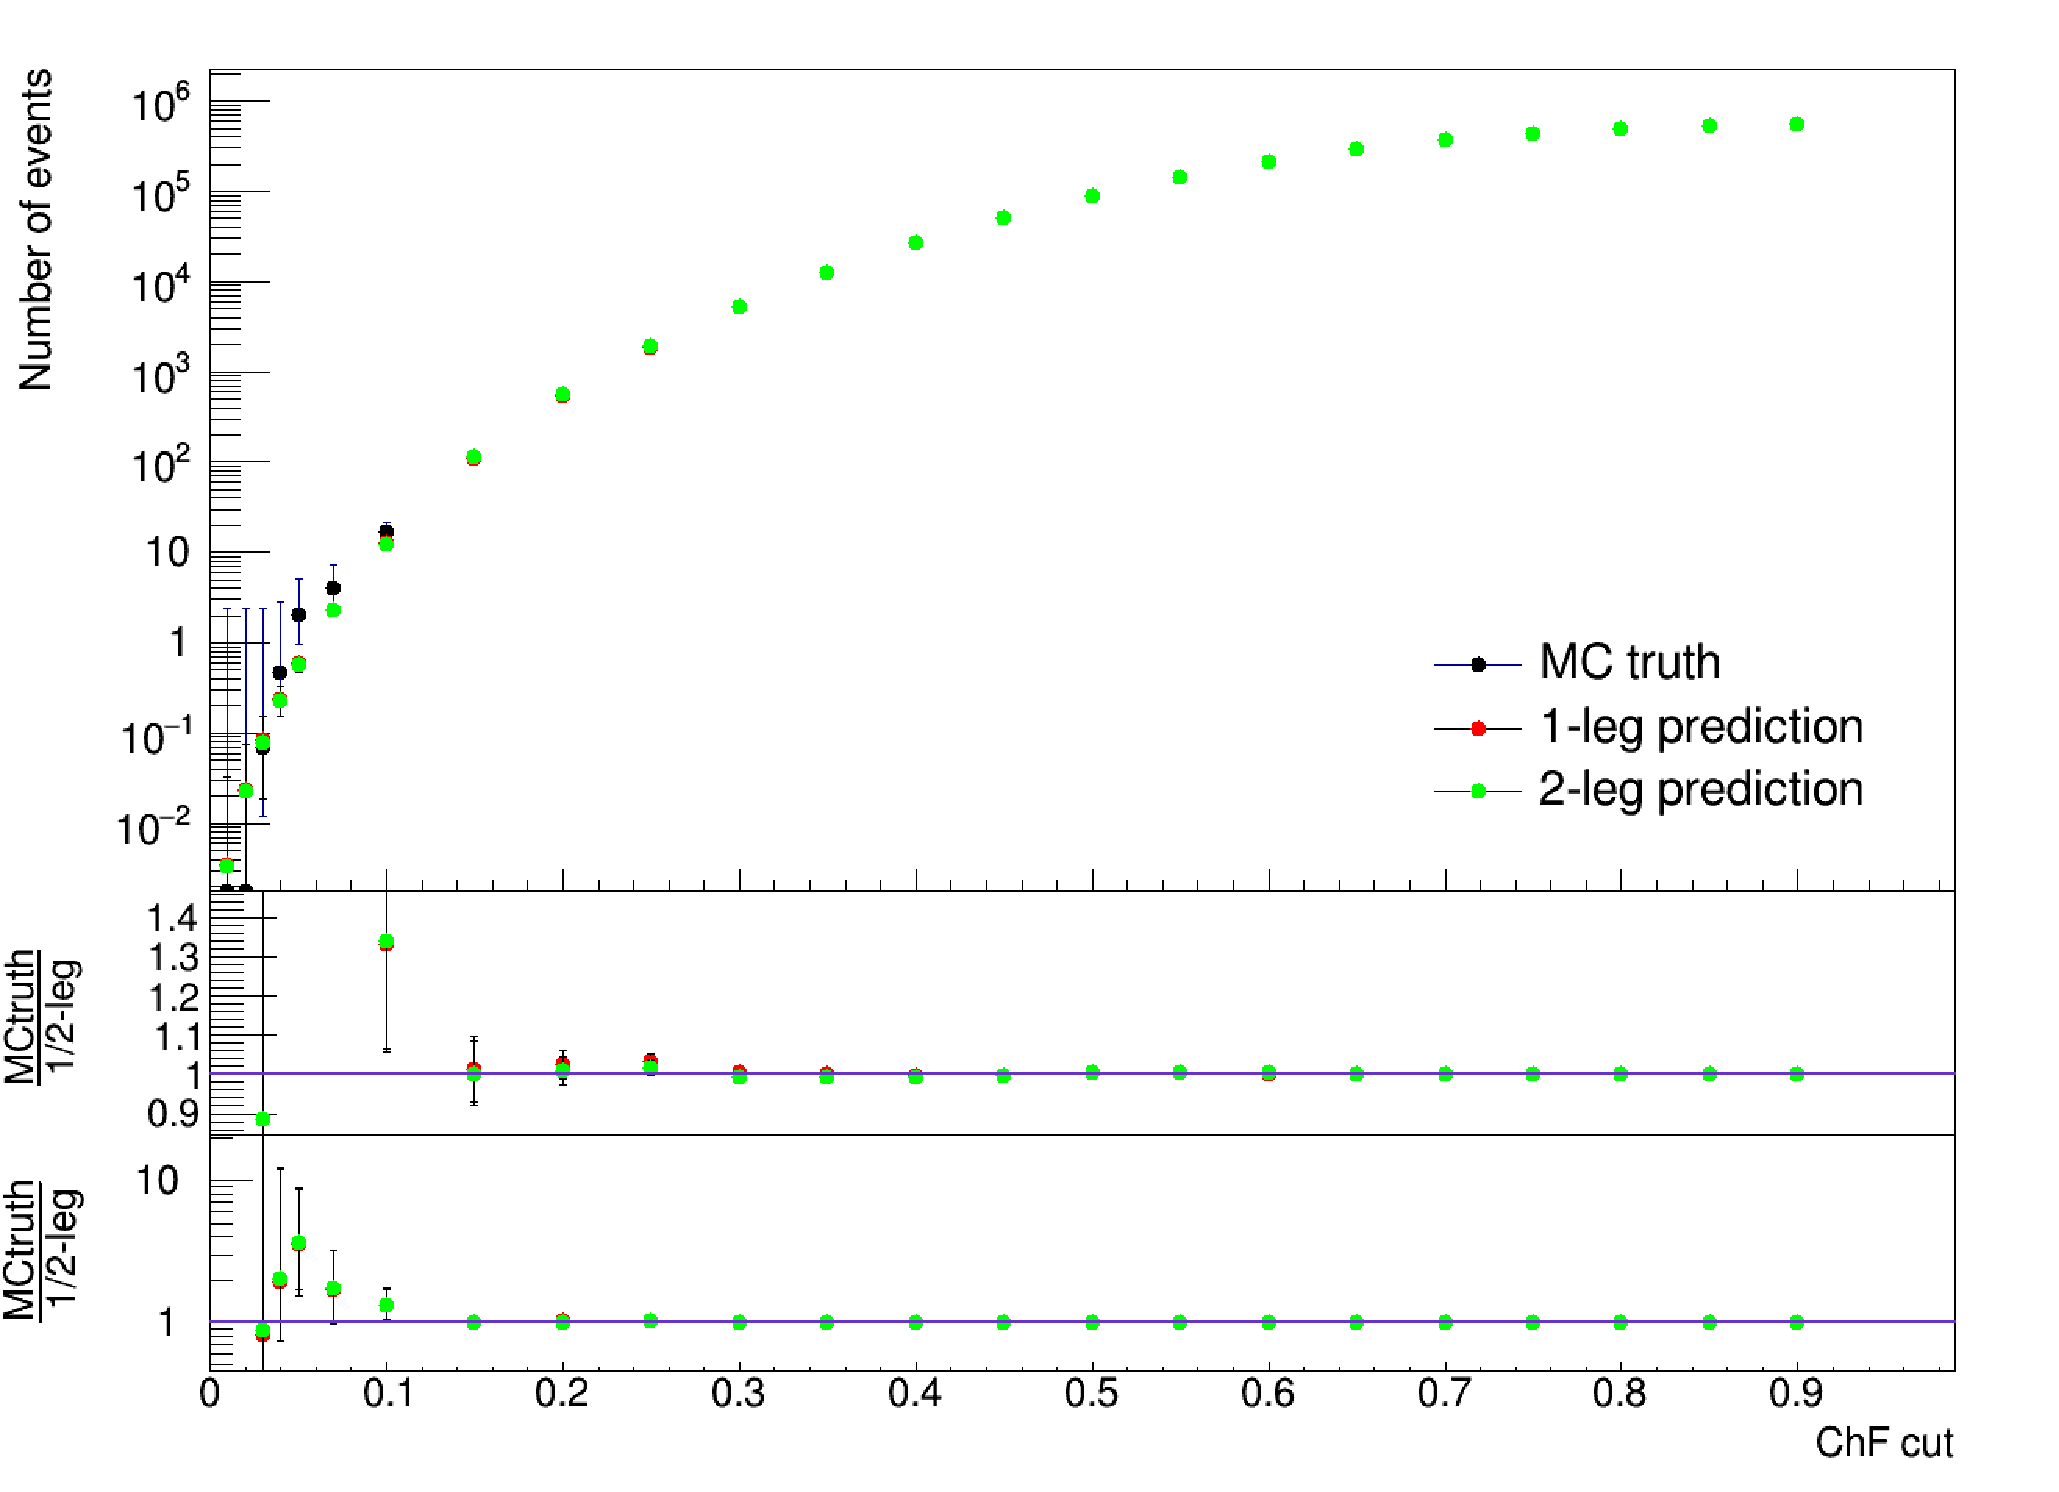
\includegraphics[width=0.48\textwidth]{figures/closure_test.pdf}\hfill
  \caption{Test of the background prediction method with simulated events, using an exclusive (left) or inclusive (right) binning in CHF. The number of events is scaled to $16.1\, \mathrm{fb}^{-1}$, corresponding to the amount of data used for this analysis.}
  \label{fig:closuretest}
\end{figure}

The \ac{QCD} background prediction in data is shown in Figure~\ref{fig:prediction} as a function of the exclusive CHF bins, using the \texttt{HLT\_PFJet450} single jet trigger. The data is blinded in the signal region below CHF = 0.05. A distinction is made between the run periods B to F (left) and G to H (right). There is a clear deviation below a CHF of 0.4 for run periods B to F, while the agreement is very good down to CHF = 0.05 for run periods G and H. The main difference between these 2 datasets is the issue with the Tracker APV pre-amplifier saturation, described in Section~\ref{sec:APVsaturation}, which was solved from run period G onwards.

\begin{figure}[ht]
  \centering
  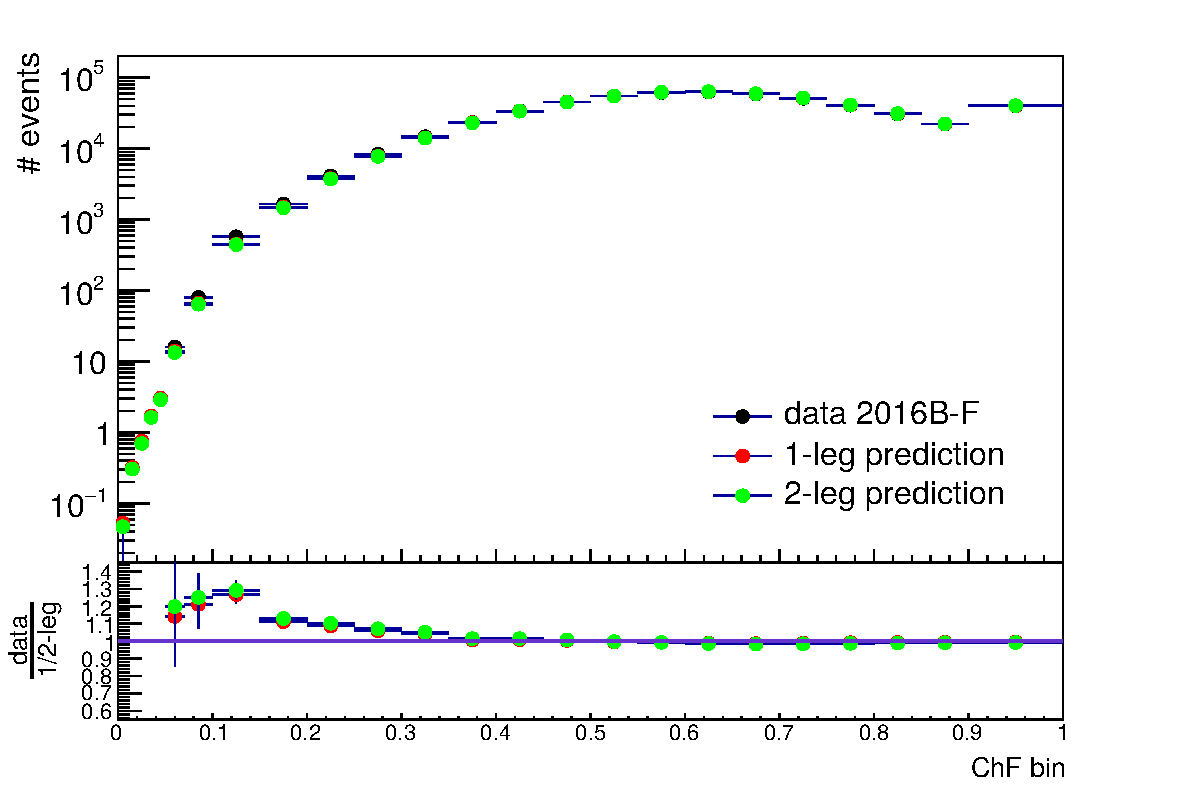
\includegraphics[width=0.5\textwidth]{figures/data_vs_prediction_BF_filters.pdf}\hfill%
  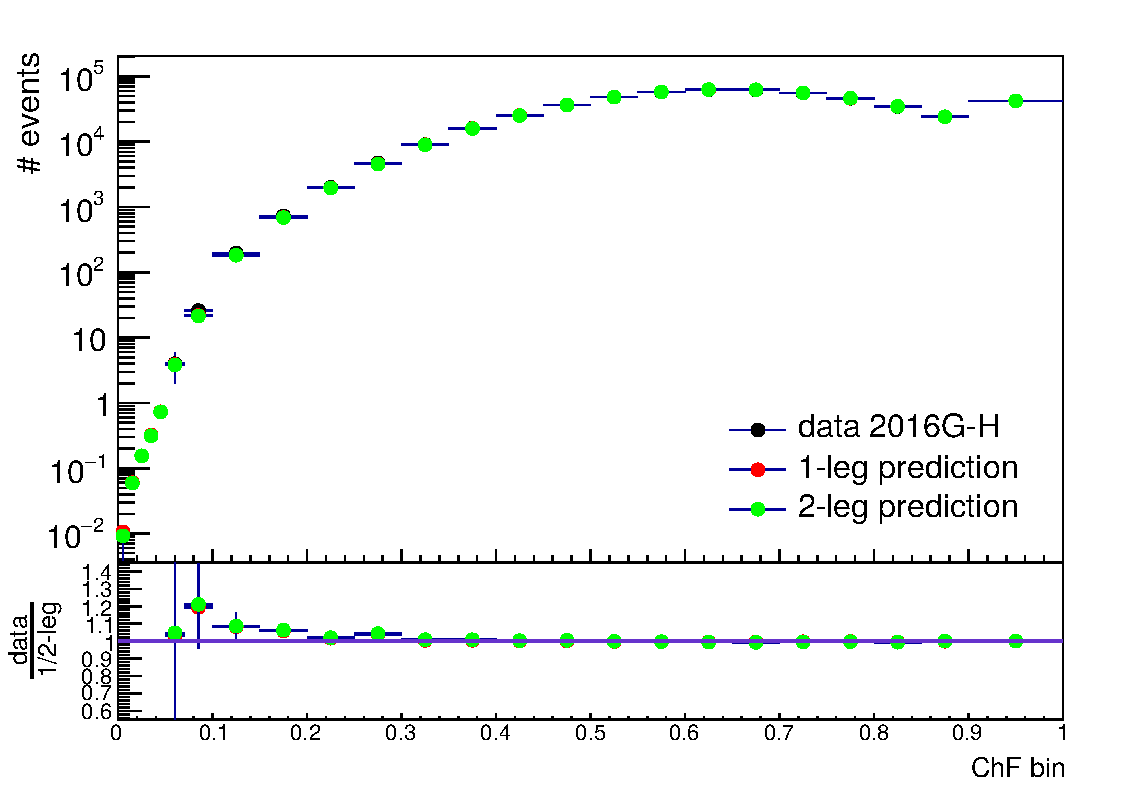
\includegraphics[width=0.5\textwidth]{figures/data_vs_prediction_GH_filters.pdf}
  \caption{The 1- and 2-leg predictions from data, as well as the data (above CHF = 0.2) as a function of the exclusive CHF bins, for run periods B-F (left) and G-H (right).}
  \label{fig:prediction}
\end{figure}

To first order, the measured CHF cut efficiencies should absorb the effects of tracking inefficiencies caused by the APV pre-amplifier saturation problem. However, this effect is also reflected in the distribution of the number of vertices. As is shown in Figure~\ref{fig:nvtx_reweighting}, a subtle effect causes the data and the prediction from data to disagree in the distribution of the number of vertices for run periods B to F, while a good agreement is obtained for run periods G to H. As there are not enough data to derive the CHF efficiencies reliably in bins of number of vertices as well as $p_T$ and $\eta$, a recovery of the data in this way is not possible. A reweighting was also performed, using a fit to the ratio of data divided by the 2-leg prediction per CHF bin. Figure~\ref{fig:BF_reweighted} shows the data versus data prediction comparison in run period E, applying the reweighting based on the number of vertices in the event, per CHF bin, and a clear improvement can be observed for the 2-leg prediction. In contrast, the 1-leg prediction has not been reweighted and still shows the original disagreement. This reweighting can however not be used in the signal region, where very few events remain. As a result, the analysis is performed with run periods G and H only, corresponding to an integrated luminosity of $16.1\,\mathrm{fb^{-1}}$. The rejected data, from run periods B to F, corresponds to an integrated luminosity of $17\, \mathrm{fb}^{-1}$.

\begin{figure}[ht]
  \centering
  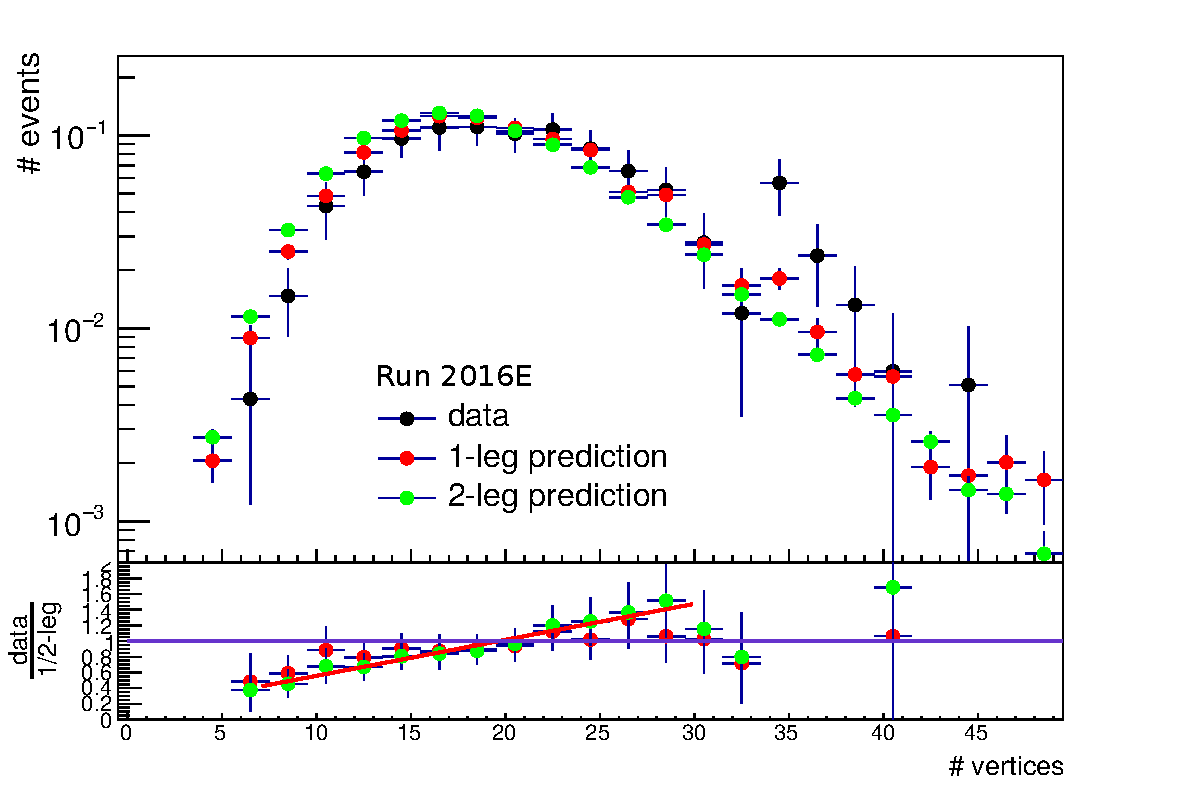
\includegraphics[width=0.5\textwidth]{figures/Data_distributions_excl_RunE_ChF0p25To0p3_nvtx.pdf}\hfill%
  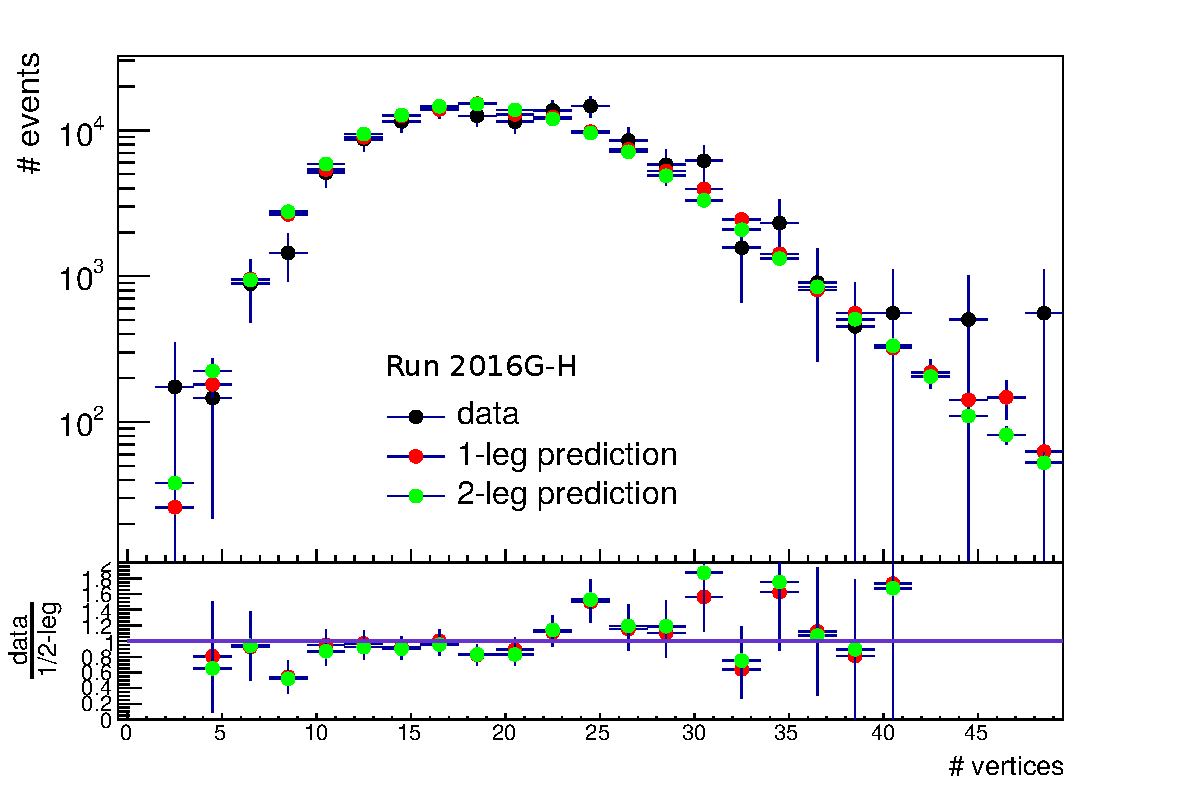
\includegraphics[width=0.5\textwidth]{figures/RunGH_ChF0p25To0p3_nvtx.pdf}
  \caption{The distribution of the number of vertices for data, 1-leg, and 2-leg prediction using data from run period E (left) and run periods G-H (right).}
  \label{fig:nvtx_reweighting}
\end{figure}

\begin{figure}[ht]
  \centering
  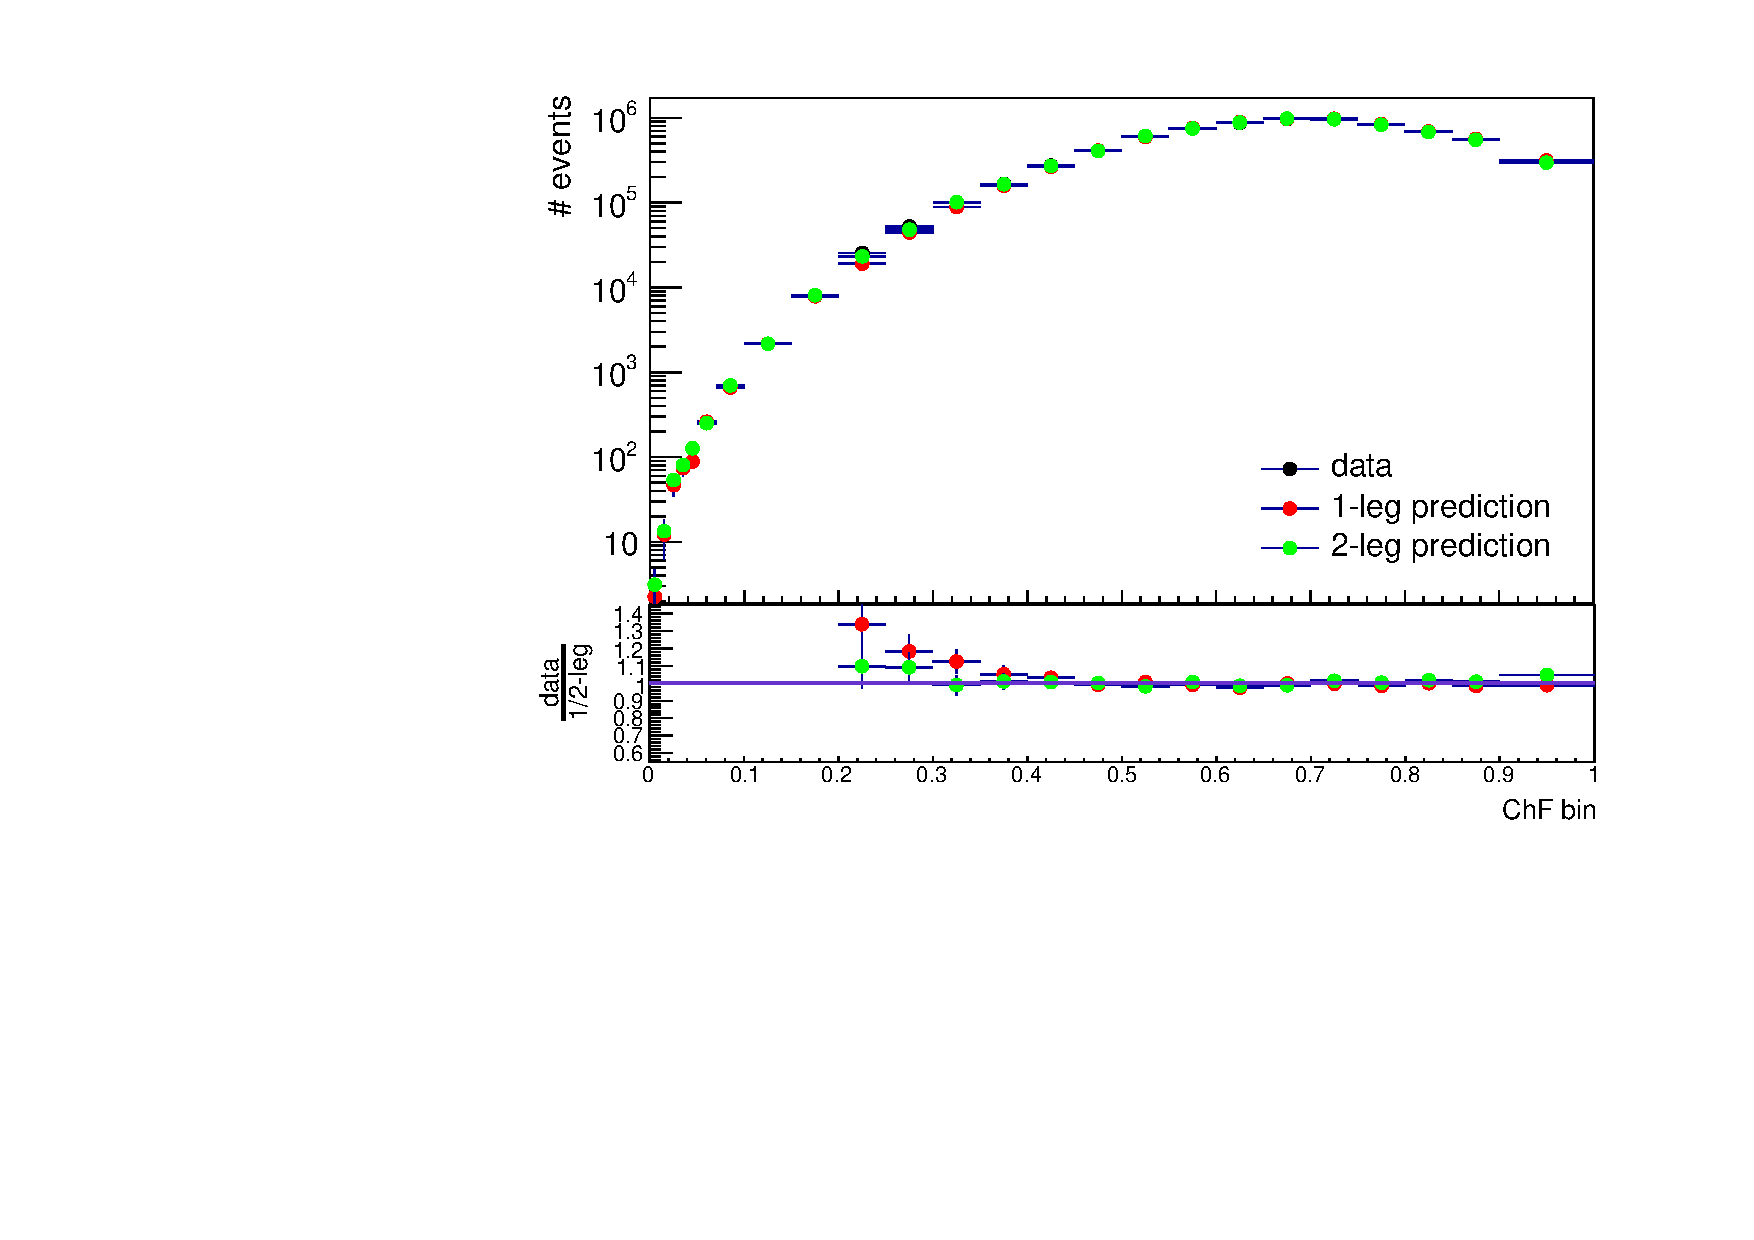
\includegraphics[width=0.7\textwidth]{figures/data_vs_prediction_RunE_reweighted_exclusivebinning.pdf}\hfill%
  \caption{The 1- and 2-leg predictions from data, as well as the data (above CHF = 0.2) as a function of the exclusive CHF bins for run period E, reweighting the 2-leg prediction to data based on the number of vertices in the event, per CHF bin.}
  \label{fig:BF_reweighted}
\end{figure}

\section{Systematic uncertainties}
\label{sec:SIMP_systematics}

For the signal prediction, systematic uncertainties are included for the luminosity, the jet energy corrections, and the trigger inefficiency. The systematic uncertainty for the luminosity amounts to 2.5\%~\cite{}. The systematic uncertainty coming from the jet energy corrections is computed by varying the jet energy by the correction and recalculating the yield after applying the selection cuts and the CHF cut. Depending on the \ac{SIMP} mass and the CHF cut, this uncertainty varies between 0.4\% and 3.9\%. A systematic uncertainty is also included to take into account the trigger inefficiency at \SI{550}{GeV} due to the turn-on. This is done by taking 100\% of the maximal inefficiency as the uncertainty, which gives a 2\% systematic uncertainty for the signal. This does not take into account the fact that the turn-on was determined for one jet only and the inefficiency is strongly reduced when two jets with a similar $p_T$ are present in the event. However, some signal events have one of the two jets with EMF = 0. In this case the jet which does not contain electromagnetic energy would not fire the single jet trigger, which requires the jet to have EMF $> 0$, and these events become single jet events from the trigger point of view. The 2\% uncertainty is therefore conservative as it represents the worst case scenario. The photon and conversion veto was found to be 100\% efficient on the signal, and as a result this systematic uncertainty is negligible. The effect of pileup was considered to be negligible as well, as the distribution of the number of vertices is very similar for the data and \ac{SIMP} samples. As an example the data is compared to the \ac{SIMP} sample with $m_{\chi} = 1000$~GeV in Figure~\ref{fig:PU}, which shows that there is a good agreement in the bulk of the distribution with some deviations for a few events with a high number of primary vertices only.

\begin{figure}[ht]
  \centering
  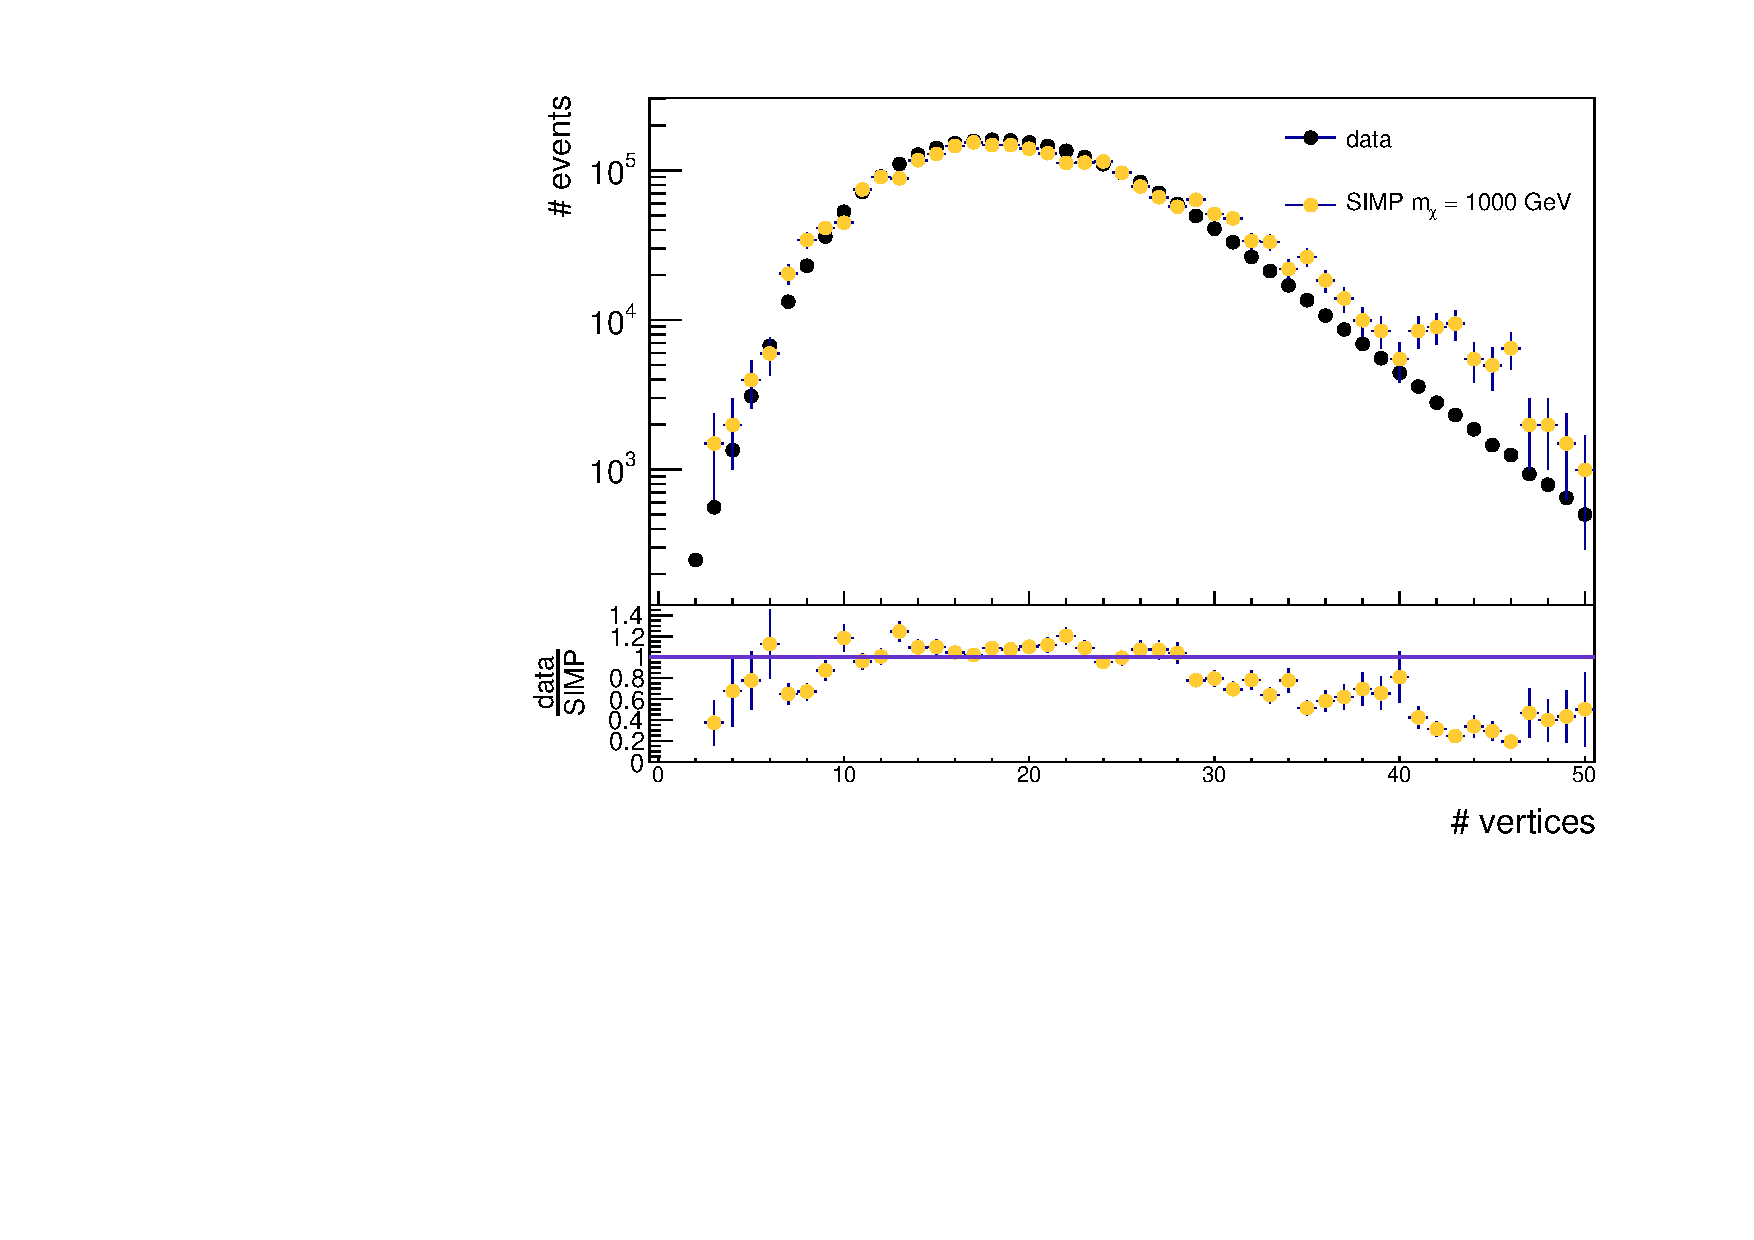
\includegraphics[width=0.7\textwidth]{figures/PU_reweighting_SIMP_M-1000.pdf}\hfill%
  \caption{The distribution of the number of vertices in data compared to the \ac{SIMP} signal with $m_{\chi} = 1000$~GeV.}
  \label{fig:PU}
\end{figure}

As mentioned in Section~\ref{sec:SIMP_backgrounds}, the main systematic uncertainty on the background prediction is obtained from the closure test in MC, by taking the difference between the MC truth and the prediction, unless it is smaller than the statistical uncertainty on the MC truth, in which case the uncertainty on the MC truth is taken as systematic uncertainty. This uncertainty varies between 4\% and 3400\%, depending on the CHF cut. As for the signal, the trigger inefficiency due to the turn-on at 550 GeV is also taken into account, yielding an additional 2\% systematic uncertainty also for the background.

\section{Results}
\label{sec:SIMP_results}

Table~\ref{tab:results} shows the number of predicted and observed events, per considered CHF cut. The prediction is done using the 1-leg data prediction, as this provides slightly smaller uncertainties, as every event can be used twice by applying the CHF first on one jet and then on the other. The statistical uncertainty, as well as the systematic uncertainty from the closure test described in Section~\ref{sec:SIMP_systematics}, are given.

A cut of $\mathrm{CHF} < 0.05$ is chosen as the final signal region selection, to reject most of the \ac{QCD} background. The background is then reduced to the level of about one event, and a large uncertainty does not have big consequences. Moreover, the uncertainty from the closure test is reduced when taking into account the smaller statistical uncertainty on the number of background events during the limit calculation. In addition, the expected sensitivity does not improve significantly at tighter CHF cuts, and the closure tests becomes statistically limited. The dominating uncertainty then comes from the closure test, and amounts to 250\% in this case.

\renewcommand{\arraystretch}{1.3}
\begin{table}[ht]
  \centering
\begin{tabular}{| c | r@{$\,\,$}r@{$\,\,$}r@{$\,\,$}r@{$\,\,$}r | r@{$\,\,$}r@{$\,\,$}r | r | r | r |}
\hline
\multirow{2}{*}{CHF cut} & \multicolumn{5}{c|}{\multirow{2}{*}{data prediction}} &  \multicolumn{3}{c|}{QCD MC} & \multirow{2}{*}{observed} & \multicolumn{2}{c |}{SIMP signal [$m_{\chi}$]} \\
\cline{11-12}
 &  &  & & & & \multicolumn{3}{c|}{prediction} & & 1 GeV & 1000 GeV\\
\hline
0.2 & 902 & $\pm$ & 5 (stat.) & $\pm$ & 38 (syst.) & 546.5  & $\pm$ & 0.6 & 969 & 634 & 4.9 \\
0.15 & 210 & $\pm$ & 2 (stat.) & $\pm$ & 18 (syst.) & 111.1  & $\pm$ & 0.4 & 229 & 634 & 4.9 \\
0.1 & 26.9 & $\pm$ & 0.3 (stat.) & $\pm$ & 8.9 (syst.) & 12.6  & $\pm$ & 0.2 & 30 & 634 & 4.9 \\
0.07 & 5.1 & $\pm$ & 0.1 (stat.) & $\pm$ & 4.4 (syst.) & 2.3  & $\pm$ & 0.2 & 4 & 634 & 4.9 \\
0.05 & 1.28 & $\pm$ & 0.03 (stat.) & \multicolumn{2}{l |}{$\!\!\!^{+\ 3.24}_{-\ 1.28\,}$ (syst.)} & 0.6  & $\pm$ & 0.1 & 0 & 634 & 4.9 \\
0.04 & 0.55 & $\pm$ & 0.02 (stat.) & \multicolumn{2}{l |}{$\!\!\!^{+\ 2.81}_{-\ 0.55\,}$ (syst.)} & 0.24  & $\pm$ & 0.09 & 0 & 633 & 4.9 \\
0.03 & 0.22 & $\pm$ & 0.01 (stat.)& \multicolumn{2}{l |}{$\!\!\!^{+\ 7.68}_{-\ 0.22\,}$ (syst.)} & 0.08  & $\pm$ & 0.07 & 0 & 632 & 4.9 \\
\hline
\end{tabular}
\caption{Number of predicted (using the 1-leg prediction from data) and observed events for several inclusive cuts on the CHF of both jets. The expected number of signal events is also given for the $m_{\chi} = 1$ GeV and $m_{\chi} = 1000$~GeV scenarios.}
\label{tab:results}
\end{table}

Model-independent limits are derived for a $\mathrm{CHF} <$ 0.05 cut, using the $CL_S$ criterion~\cite{CLS1,CLS2} with the LHC style test statistic in which the systematic uncertainties are modelled as nuisance parameters. This was done using the RooStat-based Combine tool, taking into account the  systematic uncertainties detailed in Section~\ref{sec:SIMP_systematics}, as well as the statistical uncertainties on signal and background predictions. All included systematic uncertainties are profiled with a lognormal prior, except for the uncertainty coming from the closure test, which is profiled with a gamma function since it arises from the limited number of remaining events. The resulting expected fiducial cross section is $\sigma_{\mathrm{fid}}^{95\%} = \sigma\times\mathrm{A}\times\epsilon = 0.17$~fb. With zero observed events, the observed model-independent lower limit is found to be $\sigma_{\mathrm{fid, obs}}^{95\%} = 0.18$~fb.

\section{SIMP model interpretation}
\label{sec:SIMP_interpretation}

Limits are also derived on the production cross section for the \ac{SIMP} simplified model, using the same method as described for the model-independent limits.  The expected limits on the production cross section are shown for \ac{SIMP} masses between 1 and 1000~GeV in Figure~\ref{fig:SIMP_limit}, using a cut of $\mathrm{CHF} < 0.05$. In this case, the search is sensitive to all the generated \ac{SIMP} mass points, up to 1000~GeV.

Figure~\ref{fig:SIMP_limit_unblinded} shows the expected and observed limits when including the observation of zero events in the signal region. The expected and observed limits, and the theoretical cross section are given with respect to the generator level cuts applied in the signal sample generation, $p_T^{\chi} > 200$~GeV and $|\eta_{\chi}| < 2.5$. The shown theoretical cross section is also given per \ac{SIMP} mass point in Table~\ref{tab:signal_samples}. In summary, no significant excess above the expected background is observed, and the considered \ac{SIMP} simplified model is ruled out for \ac{SIMP} masses up to 1000~GeV.

\begin{figure}[ht]
  \centering
  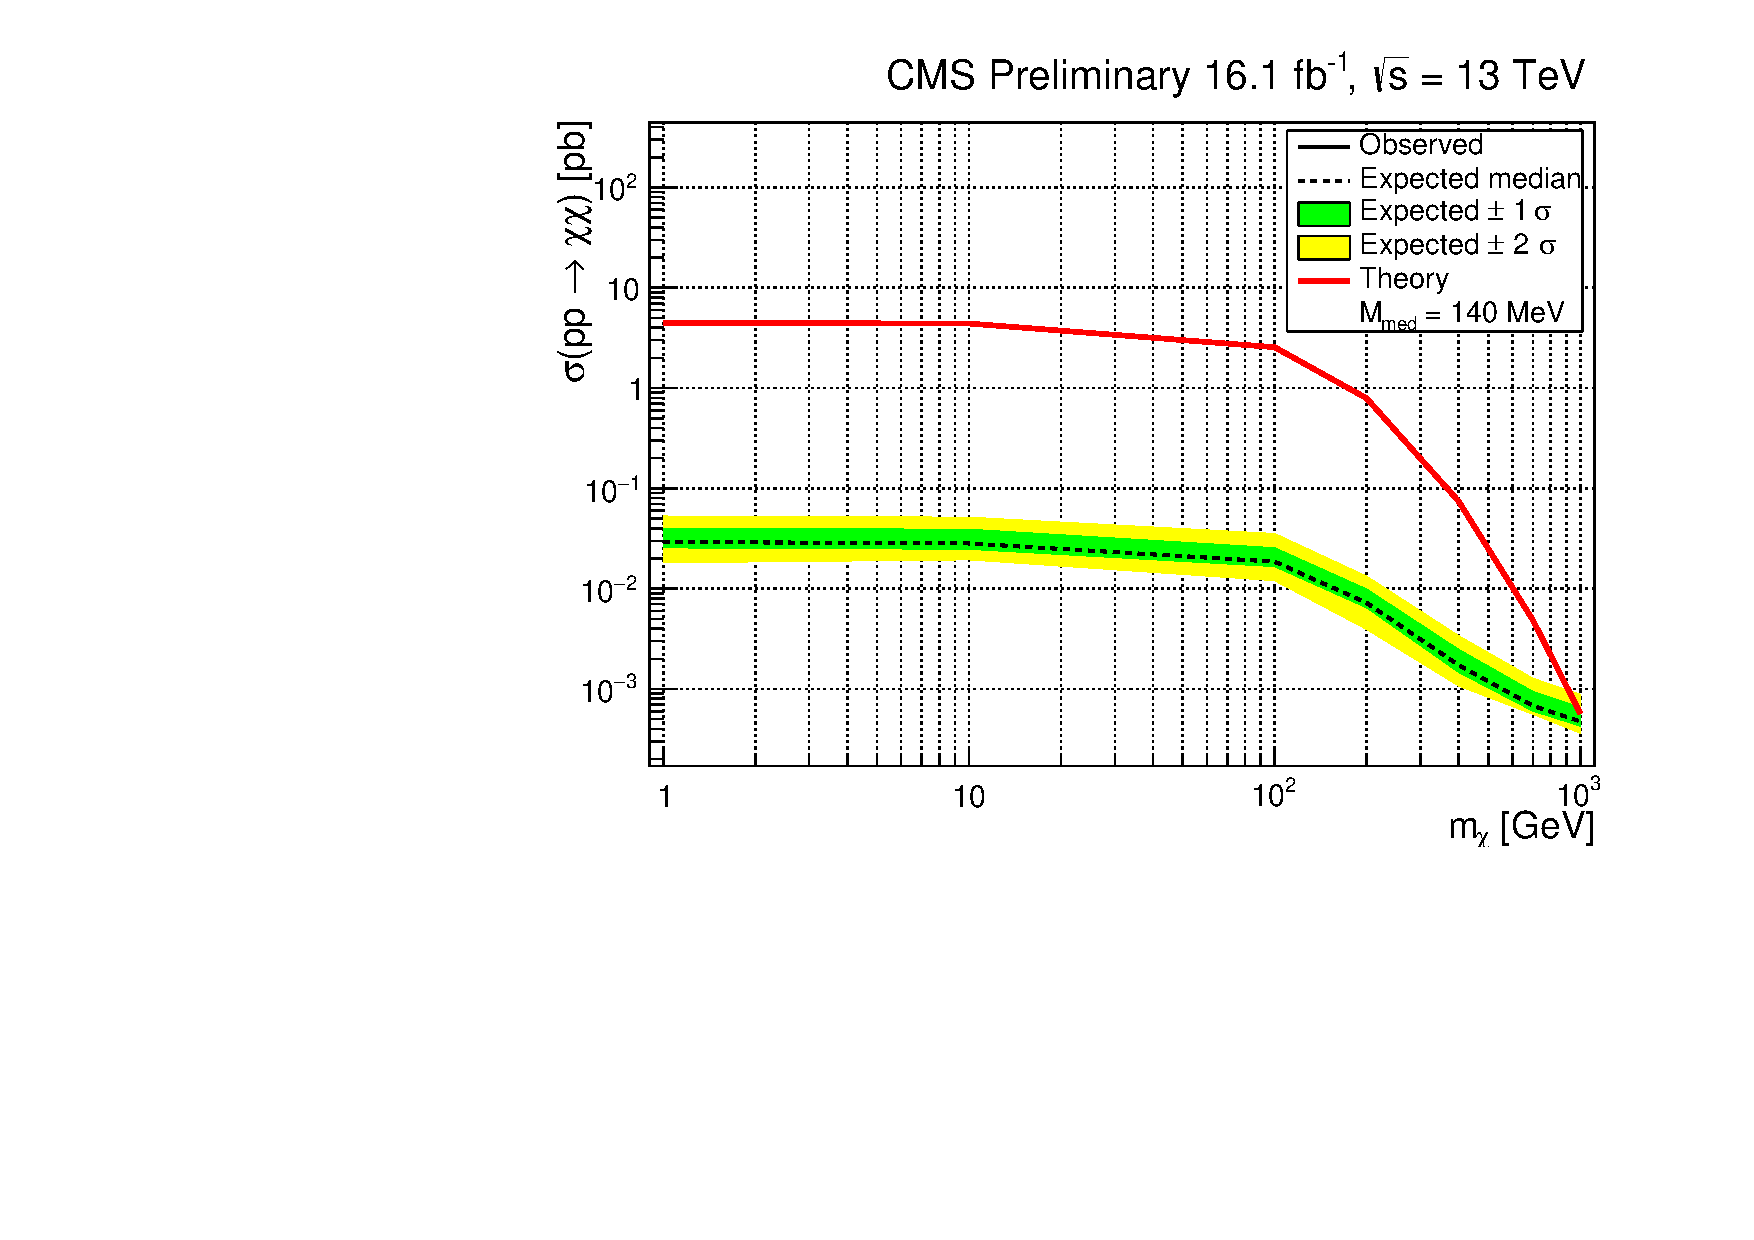
\includegraphics[width=0.8\textwidth]{figures/SIMP_limit_ChF0p05.pdf}\hfill%
  \caption{The expected limits on the production cross section, obtained without looking in the signal region, for \ac{SIMP} masses between 1 and 1000~GeV, with $1\sigma$ and $2\sigma$ bands is shown, as well as the theoretical prediction (red), with respect to the generator level cuts ($p_T^{\chi} > 200$~GeV and $|\eta_{\chi}| < 2.5$).}
  \label{fig:SIMP_limit}
\end{figure}

\begin{figure}[ht]
  \centering
  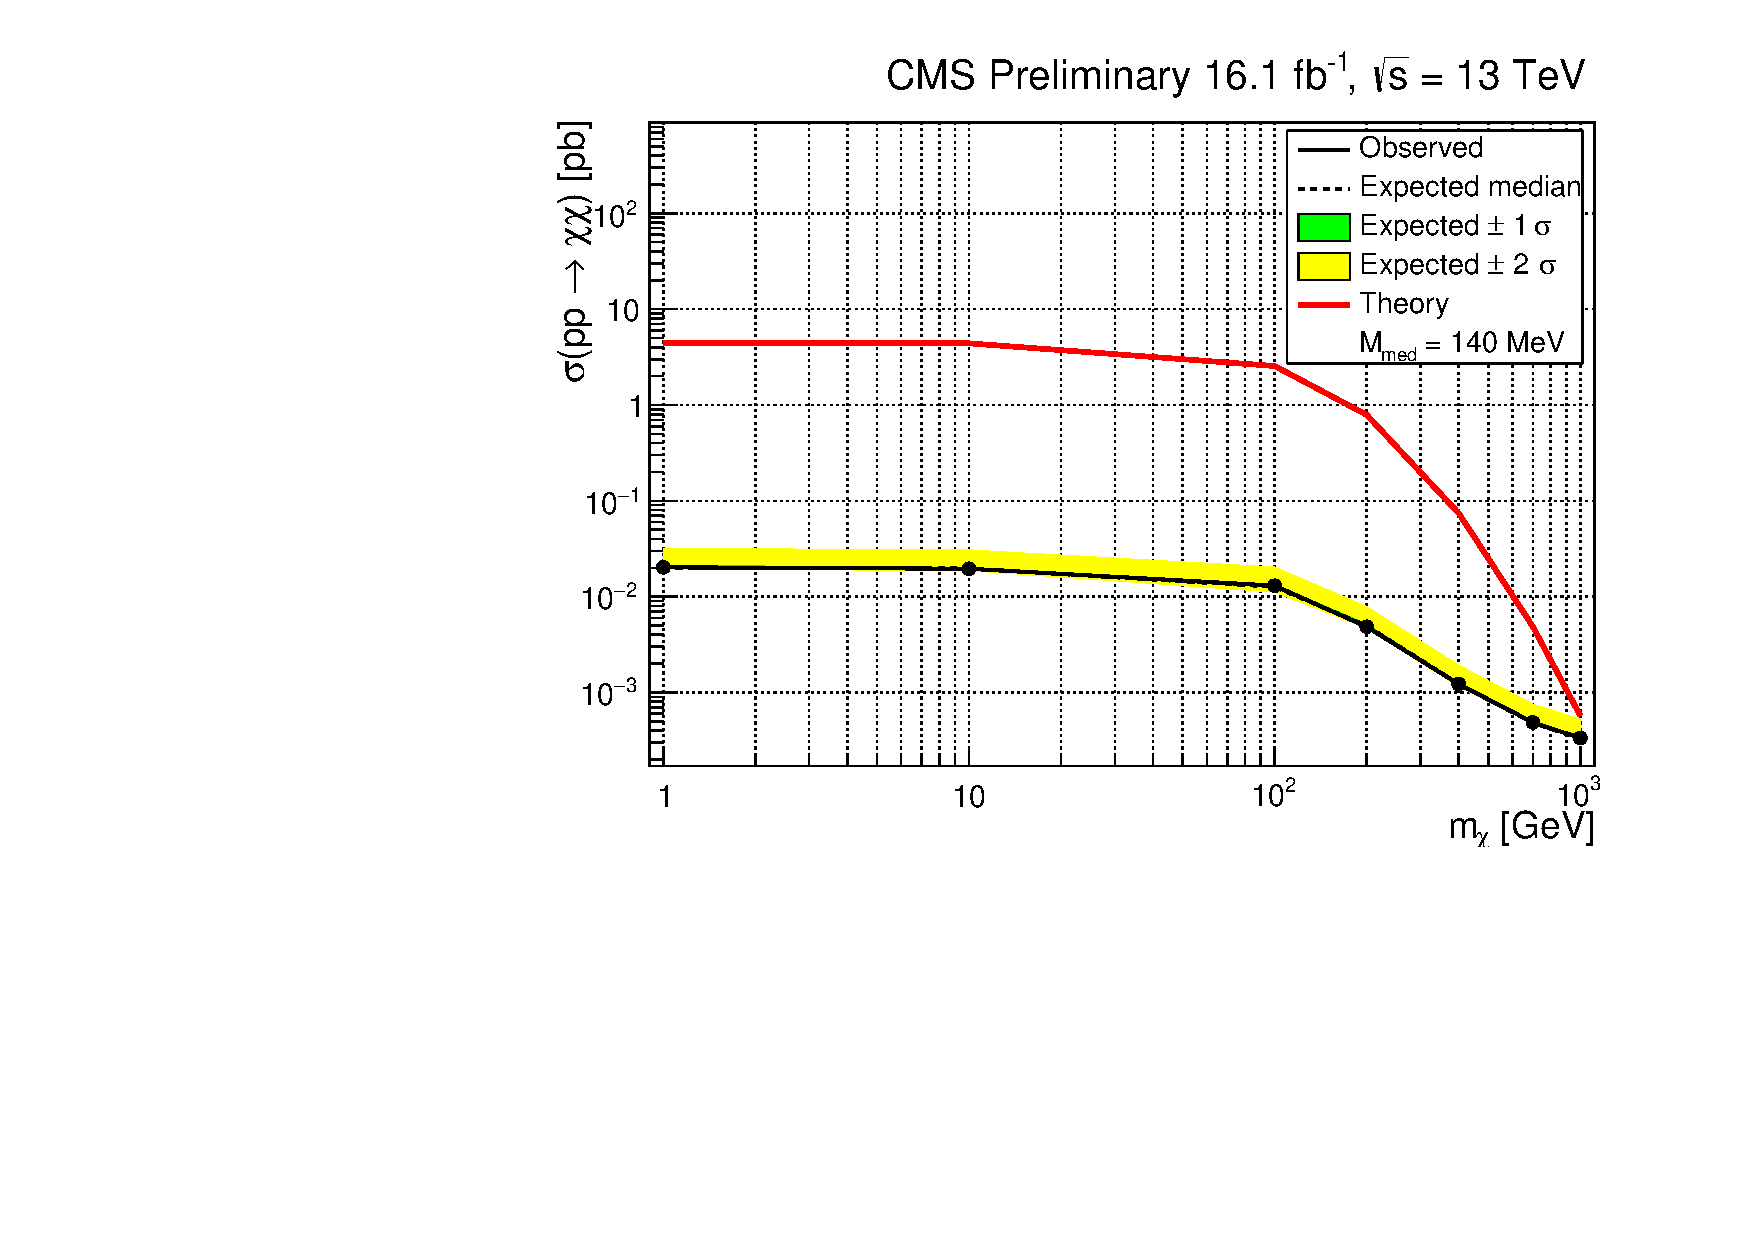
\includegraphics[width=0.8\textwidth]{figures/SIMP_limit_ChF0p05_unblinded.pdf}\hfill%
  \caption{The expected and observed limits on the production cross section for \ac{SIMP} masses between 1 and 1000~GeV, with $1\sigma$ and $2\sigma$ bands is shown, as well as the theoretical prediction (red), with respect to the generator level cuts ($p_T^{\chi} > 200$~GeV and $|\eta_{\chi}| < 2.5$).}
  \label{fig:SIMP_limit_unblinded}
\end{figure}

\clearpage


\clearpage{\pagestyle{empty}\cleardoublepage}
